\section{\prob{} Solution}\label{sec:sol}
In this section,  we first present the $\vats$ algorithm as a solution to \prob{} and propose techniques to optimize its efficiency in Section~\ref{sec:greedy}.
Then we improve $\vats$ with an advanced algorithm $\vatss$ by considering trajectory data distribution and human perception capability in Section~\ref{subsec:VQGS+}.


\subsection{Visual Quality Guaranteed Sampling $\vats$}\label{sec:greedy}
%Due to the hardness of Problem~\ref{prob:def}, the straight-forward solution is uniform random sampling $\rand$.
%This solution randomly selects $k$ trajectories from the dataset $\D$ and stores them in the result set $\oR$. The selected trajectories in $\oR$ are rendered as the visualization result.
%Obviously, uniform random sampling $\rand$ does not provide any guarantee on the visual quality of the sampled set.

Our visual quality guaranteed sampling method ($\vats$) is presented in Algorithm~\ref{alg:greedy},
which takes the trajectory dataset $\D$ and a sampling rate $\alpha$ as input (i.e., $k=\lceil \alpha |\mathcal{T}| \rceil$).
$\vats$ employs a greedy paradigm and finds the trajectory $\mathsf{tmp}$ in $\D$ that maximizes $| \mathsf{tmp} \cup \VV(\oR)|$ at each iteration, as shown in Line~\ref{line:max} of Algorithm~\ref{alg:greedy}.
It terminates after $k=\lceil \alpha |\mathcal{T}| \rceil$ iterations and returns $\oR$ as the result set.
As the visualization quality $\QQ(\mathcal{R})$ can be computed after each iteration in Algorithm~\ref{alg:greedy} with pre-computed ground-truth $\VV(\mathcal{T})$,
alternatively, we can terminate the algorithm when $\VV(\mathcal{R})\ge \tau$, in which $\tau$ is the quality threshold.

\begin{algorithm}
    \caption{$\vats(\D, k=\lceil \alpha |\mathcal{T}| \rceil$)} \label{alg:greedy}
    \begin{algorithmic}[1]
    \State Initialize the result set $\oR \leftarrow \emptyset$
    \While{$|\oR| < k$}
        \State $\mathsf{tmp} \leftarrow \arg\max_{t_i \in \D} |t_i \cup \VV(\oR)|$ \label{line:max}
        \State $\oR \leftarrow \oR \cup \{ \mathsf{tmp} \}$
    \EndWhile
    \State Return $\oR$
    \end{algorithmic}
\end{algorithm}

Algorithm~\ref{alg:greedy} provides provable visual quality guarantee for the result set $\oR$, as stated in Theorem~\ref{the:ratio}.

\begin{theorem}~\label{the:ratio} Given a sample rate $\alpha$, and let the optimal solution to \prob{} defined in Equation~\eqref{eq:opp} be $\mathcal{R}^{\star}$ and the solution provided by Algorithm~\ref{alg:greedy} be $\mathcal{R}$, we have $\QQ(\mathcal{R})\ge 0.632*\QQ(\mathcal{R}^{\star})$.
\end{theorem}

Theorem~\ref{the:ratio} follows directly from the submodularity of the visualization quality function $\QQ(\mathcal{R})$,
and it is well known that greedy solution provides a $0.632$ approximation of the optimal solution for a submodular function~\cite{fujishige2005submodular}.
As $\QQ(\mathcal{R})$ is simply a linear scaling of $|\VV(\oR)|$ as shown in Equation~\eqref{eqn:obj2}, we prove  $|\VV(\oR)|$ is submodular as follows.

\begin{lemma}[Submodularity]\label{lem:submodular}
Define the contribution value of a trajectory $t$ to a sample set $\oR$ as $\Delta(\oR, t) = |\VV(\oR \cup t)| - |\VV(\oR)|$.
Given a trajectory $t$ and two sample sets $\oR,\oR^{'}$, if $\oR \subset \oR^{'}$, then $ \Delta(\oR, t) \geq \Delta(\oR^{'}, t)$.
\end{lemma}

\begin{proof}
The contribution value of trajectory $t$ w.r.t. a given result set $\oR$ (i.e., $\Delta(\oR, t) = |\VV(\oR \cup t)| - |\VV(\oR)|$) is the number of pixels covered by $t$ but not the trajectory set $\oR$,
which can be expressed as $|\VV(t)| - |\VV(\oR) \cap \VV(t))|$.
We have $\VV(t) \cap \VV(\oR) \subseteq \VV(t) \cap \VV(\oR^{'}) $ because $\oR^{'}$ is a superset of $\oR$, which implies $|\VV(t)| - |\VV(\oR) \cap \VV(t))| \geq |\VV(t)| - |\VV(\oR^{'})\cap \VV(t))|$.
Thus, it holds that $\Delta(\oR, t) = |\VV(\oR \cup t)| - |\VV(\oR)| \geq |\VV(\oR^{'} \cup t)| - |\VV(\oR^{'})|= \Delta(\oR^{'}, t)$.
\end{proof}


%\begin{proof}
%The optimal solution of Problem~\ref{prob:def} covers $f(\mathcal{R}^{\star})$ pixels in $k$ iterations.
%Let $a_i$ be the number of newly covered pixels at the $i$-th iteration, $b_i$ is the total number of covered pixels up to the $i$-th iteration (i.e., $b_i = \sum_{j=1}^{i}a_i$),
%and $c_i$ be the uncovered pixels after $i$-th iteration (i.e., $c_i = f(\mathcal{R}^{\star})-b_i$).
%According to greedy paradigm, we can conclude the number of newly covered pixels at the $(i+1)$-th iteration is always greater than or equal to $\frac{1}{k}$ of the number of uncovered pixels after the $i$-th iteration, i.e., $a_{i+1} \geq \frac{c_i}{k}$.
%We prove Theorem~\ref{the:ratio} by proving $c_{i+1} \leq (1-1/k)^{i+1} \cdot f(\mathcal{R}^{\star})$.
%It holds $c_1 \leq (1-1/k) \cdot f(\mathcal{R}^{\star})$ as follows.
%\begin{align} \nonumber
%& a_1 \geq c_0 \cdot 1/k = 1/k \cdot f(\mathcal{R}^{\star}) \text{~~~as we concluded~~~} a_{i+1} \geq \frac{c_i}{k}\\ \nonumber
% \Leftrightarrow  & b_1 \geq 1/k \cdot f(\mathcal{R}^{\star})  \Leftrightarrow  -b_1 \leq - 1/k \cdot f(\mathcal{R}^{\star})  \text{~~~as~~~} a_1 = b_1\\ \nonumber
% \Leftrightarrow & f(\mathcal{R}^{\star}) - b_ 1 \leq f(\mathcal{R}^{\star}) - 1/k \cdot f(\mathcal{R}^{\star})  \Leftrightarrow  c_1 \leq (1-1/k) \cdot f(\mathcal{R}^{\star})
%\end{align}
%For inductive hypothesis assume $c_{i} \leq (1-1/k)^i \cdot f(\mathcal{R}^{\star})$. Thus,
%\begin{align} \nonumber
%& c_{i+1} = c_i - a_{i+1} \leq c_i - c_i/k = (1-1/k) \cdot c_i =  (1-1/k)^{i+1} \cdot f(\mathcal{R}^{\star})
%\end{align}
%
%Hence, it holds $c_k \leq (1-1/k)^{k} \cdot f(\mathcal{R}^{\star})$.
%It is equivalent to $b_k = f(\mathcal{R}) \geq (1 - (1-1/k)^{k}) \cdot f(\mathcal{R}^{\star}) \geq (1-1/e) \cdot f(\mathcal{R}^{\star}) \approx 0.632 \cdot f(\mathcal{R}^{\star})$.
%\end{proof}


Although Algorithm~\ref{alg:greedy} provides quality guarantee for the result set $\oR$, it has a high time complexity, which we show in the following analysis.

%With the above theoretical analysis, Algorithm~\ref{alg:greedy} offers a visual quality-guaranteed sampling algorithm for the large-scale trajectory data visualization problem.
%However, as the time complexity analyzed in Lemma~\ref{lem:cost}, it is not scalable to large-scale trajectory datasets (e.g., millions of trajectories).


\begin{lemma}[Time Complexity]~\label{lem:cost}
For a trajectory dataset $\D$ and an integer $k=\lceil \alpha |\mathcal{T}| \rceil$, the time complexity of Algorithm~\ref{alg:greedy} is $O(\alpha \cdot m \cdot |\D|^2)$,
where $m$ is the maximum length for the trajectories in dataset $\D$.
\end{lemma}


\begin{proof}
In each iteration, Algorithm~\ref{alg:greedy} computes the trajectory with the largest number of uncovered pixels in dataset $\D$.
It take $O(m)$ cost to compute the number of uncovered pixels for each trajectory in $\D$.
Algorithm~\ref{alg:greedy} runs for $k=\lceil \alpha |\mathcal{T}| \rceil$ iterations.
Hence, the total cost is $O(k \cdot m \cdot |\D|)=O(\alpha \cdot m \cdot |\D|^2)$.
\end{proof}

The high complexity of Algorithm~\ref{alg:greedy} hurts its scalability for large-scale trajectory datasets.
% even though sampling is conducted in the offline index building phase for CheetahTraj.
For example, the \pt{} dataset contains 2.39 millions taxi trajectories, Algorithm~\ref{alg:greedy} takes 413.6 seconds to obtain the result set $\oR$ with sampling rate $0.1\%$.

%and the longest trajectory has 3,490 GPS points
%Obviously, the running time is too long for interactive trajectory exploration.

\begin{figure}
	\centering
	\small
	\begin{tabular}{cc}
		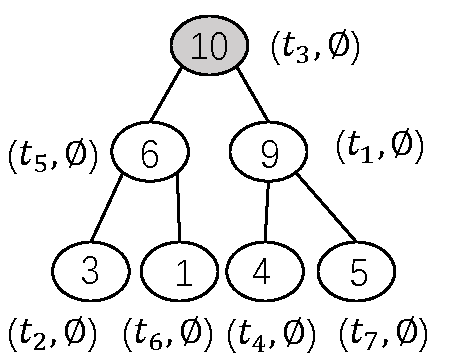
\includegraphics[width=0.4\columnwidth]{pictures/1st}
		&
		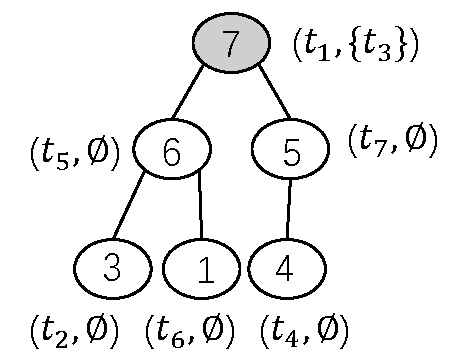
\includegraphics[width=0.4\columnwidth]{pictures/2nd}
		\\
		(A) 1st iteration
		&
		(B) 2nd iteration
	\end{tabular}
    \trim
	\caption{Heap-based lazy computation.} \label{fig:heap} %via the submodularity in Lemma~\ref{lem:submodular}
    \trim \trim
\end{figure}


\stitle{Heap-based lazy Computation}
Algorithm~\ref{alg:greedy} essentially adds the trajectory that maximizes $\Delta(\oR, t) = |\VV(\oR \cup t)| - |\VV(\oR)|$ to $\oR$ in each iteration.
Lemma~\ref{lem:submodular} shows that the contribution of a trajectory (i.e., $\Delta(\oR, t)$) cannot increase when Algorithm~\ref{alg:greedy} runs for more iterations because $ \Delta(\oR^{'}, t) \le \Delta(\oR, t) $ for  $\oR \subset \oR^{'}$.
For example, the contribution of $t_1$ is $9$ at the first iteration (i.e., $\oR = \emptyset$), see Figure~\ref{fig:heap}(a).
Its contribution turns $7$ when $\oR = \{ t_3 \}$ at the second iteration, as shown in Figure~\ref{fig:heap}(b).
Based on this property, we can use  $\Delta(\oR, t)$ calculated in the previous iterations to prune it from contribution computation.
Specifically, if we have $\Delta(\oR, t) \le \Delta(\oR^{'}, t')$, in which $\oR$ and $\oR^{'}$ are a previous and the current sample set, respectively,
we know that $t$ can not be added to the sample set in the current iteration as $\Delta(\oR^{'}, t)\le \Delta(\oR^{'}, t')$ and $t'$ is a better choice.
As shown in Figure~\ref{fig:heap}(b), even we do not know $\Delta(\oR'=\{t_3\}, t_7)$ exactly,
we can conclude $t_7$ will not be the sample set in the second iteration as $\Delta(\oR = \emptyset, t_7) = 5 < \Delta(\oR'=\{t_3\}, t_1) = 7$.


To implement this idea, we maintain a max-heap for the number of uncovered pixels in each trajectory and update the contribution of a trajectory only when necessary, i.e., computing in a lazy manner.

Consider a tiny example with 7 trajectories, i.e., $t_1$ to $t_7$.
Figure~\ref{fig:heap}(a) shows the initial max-heap and the contributions of trajectories $t_1$ to $t_7$ w.r.t result set $\oR = \emptyset$.
At the first iteration, the root node of the max-heap, $t_3$ in Figure~\ref{fig:heap}(A), is selected.
At the second iteration, the number of uncovered pixels of the new root node $t_1$ is updated to 7 w.r.t. result set $\oR = \{ t_3 \}$ (see the gray node in Figure~\ref{fig:heap}(B)).
Then $t_1$ is selected at the second iteration without computing the contributions of other trajectories w.r.t $\oR = \{ t_3 \}$.
The reason is that the contributions of these trajectories are all less than 7 when $\oR = \emptyset$,
according to the submodularity in Lemma~\ref{lem:submodular}, their contributions must be smaller than $7$ when $\oR = \{ t_3 \}$.
The efficiency of Algorithm~\ref{alg:greedy} is significantly improved with heap-based lazy computation.
Recall that Algorithm~\ref{alg:greedy} takes 413.6 seconds with sampling rate $0.1\%$ on the \pt{} dataset while our performance-optimized $\vats$ needs only 1.2 seconds.

%In summary, the number of uncovered pixels in each trajectory will only be computed with the latest result set $\oR$ when it is necessary in the lazy computing manner,
%e.g., only $t_1$ will be updated at the 2nd iteration in Figure~\ref{fig:heap}.
%It reduces many unnecessary computations through the lazy updating manner, e.g., all white nodes did not update at the 2nd iteration in the above example.

%We then analyze the time complexity of Algorithm~\ref{alg:greedy} with lazy computing manner in Theorem~\ref{lem:lazy}.
%
%\begin{lemma}[Optimized Time Complexity]~\label{lem:lazy}
%Given trajectory dataset $\D$ and an integer $k= \alpha |\D|$, the time complexity of Algorithm~\ref{alg:greedy} with lazy computing manner is $O(\alpha \cdot m \cdot x |\D| \log |\D|)$, where $x$ is the number of contribution computations among all $k$ iterations and $x \ll |\D|$.
%\end{lemma}
%
%\begin{proof}
%It first takes $O(|\D|)$ time to construct the max-heap~\cite{cormen2009introduction}.
%It incurs $O( m \cdot x \log |\D|)$ cost to select the trajectory with maximum uncovered pixels at each iteration ($k$ iterations in total).
%Hence, the overall cost is $O(|\D| + k \cdot m \cdot t \log |\D|)$.
%\end{proof}

\subsection{Advanced Approach $\vatss$}\label{subsec:VQGS+}

\begin{figure*}
   \begin{minipage}{0.7\textwidth}
     \centering
     \begin{tabular}{ccc}
     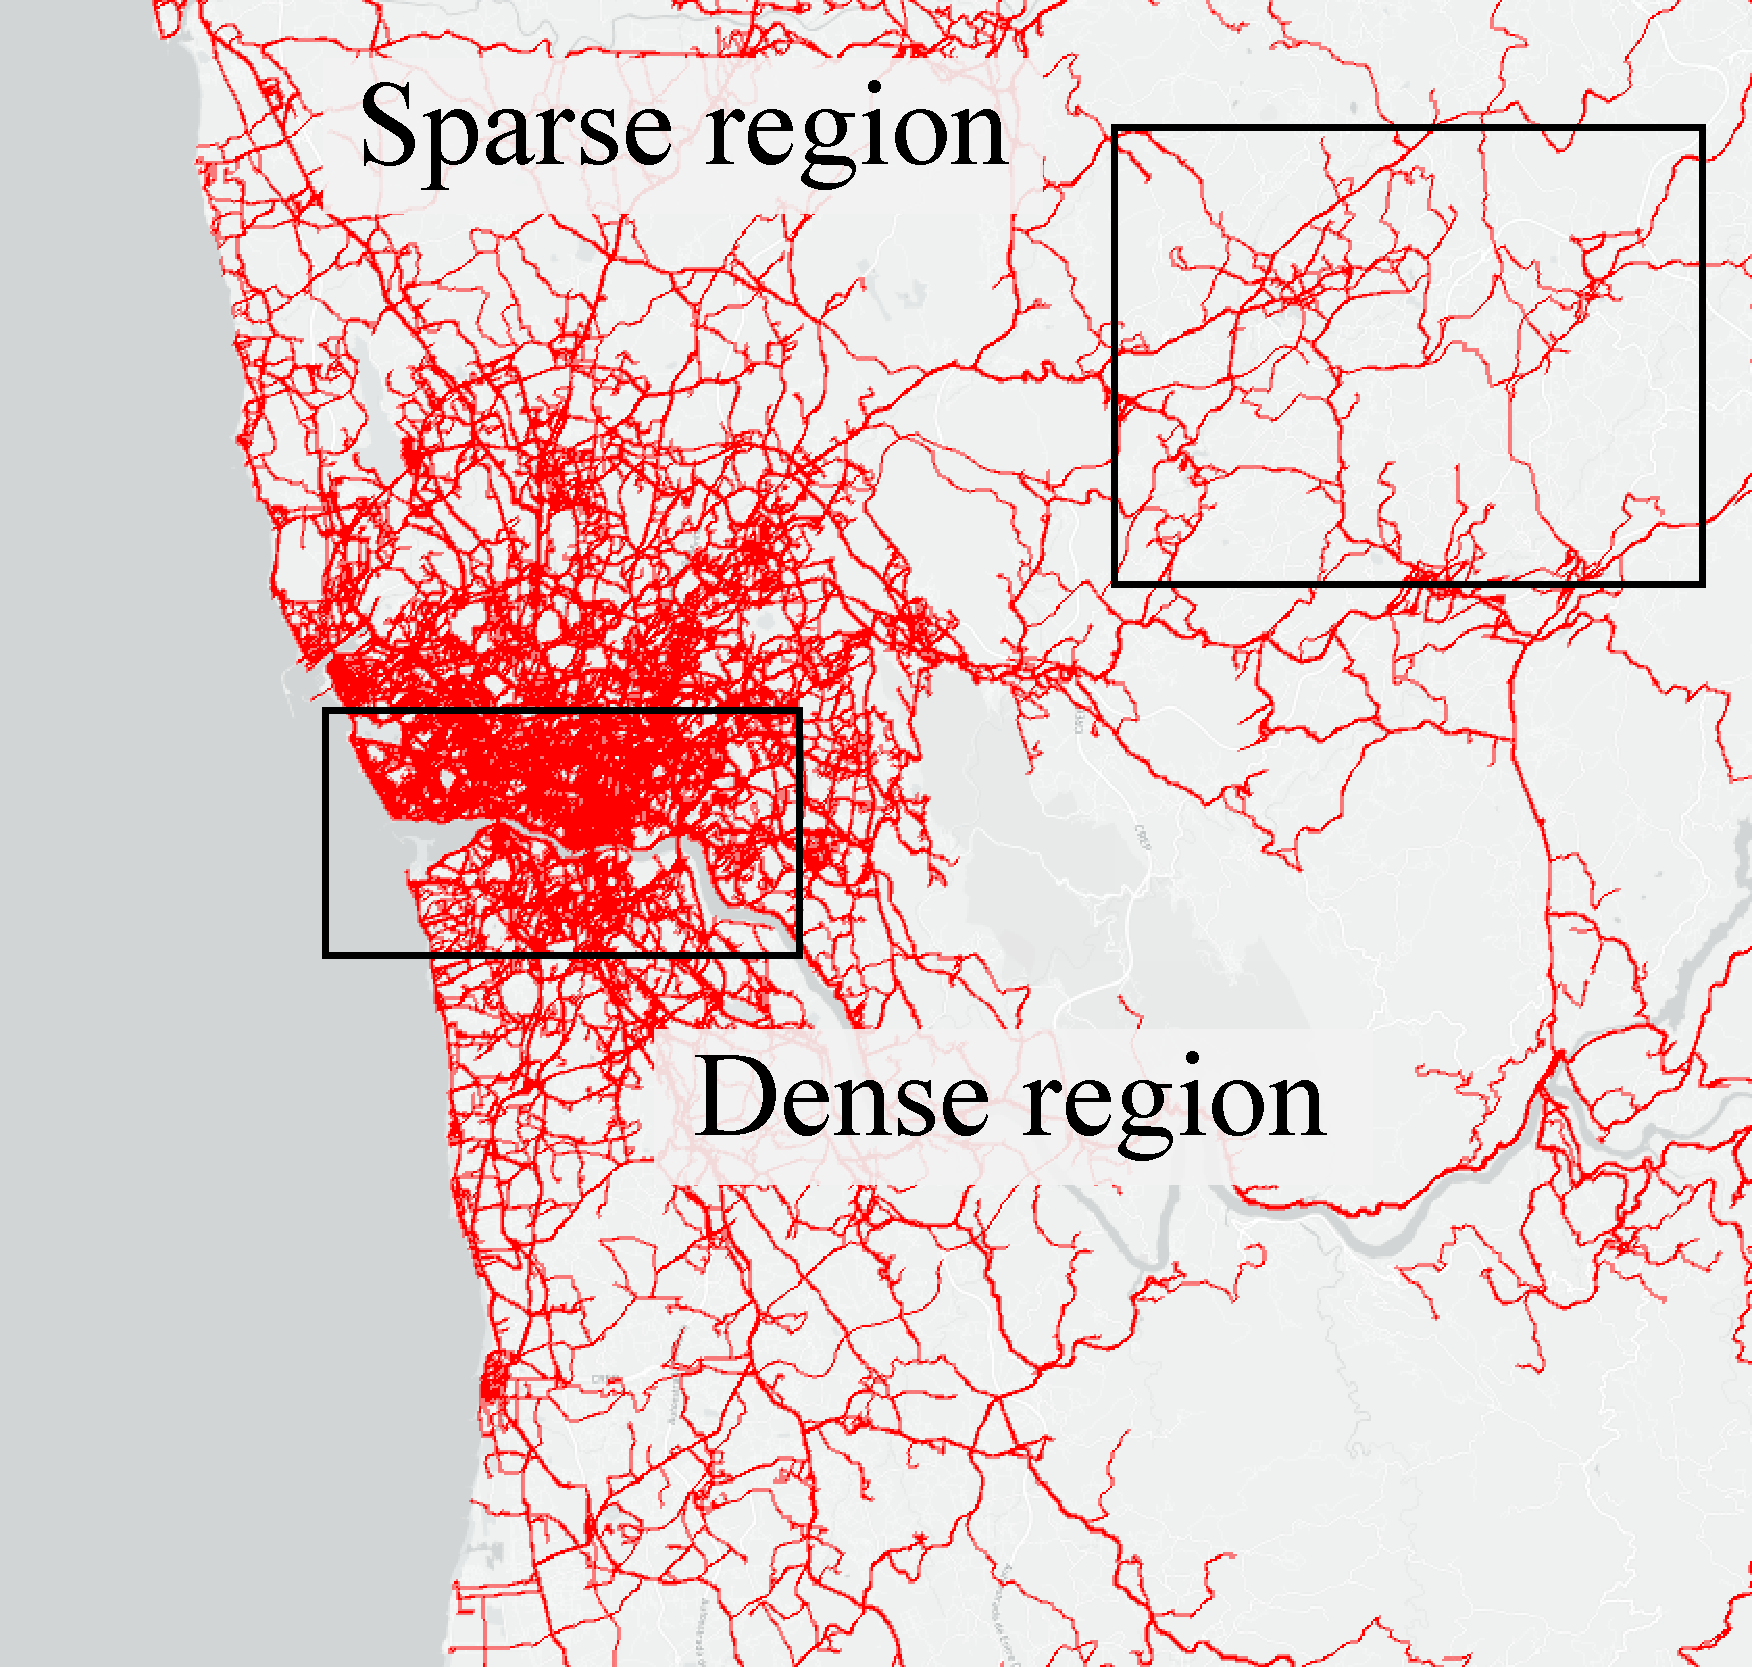
\includegraphics[width=0.250\linewidth]{pictures/motivation_VQGS}
     &
     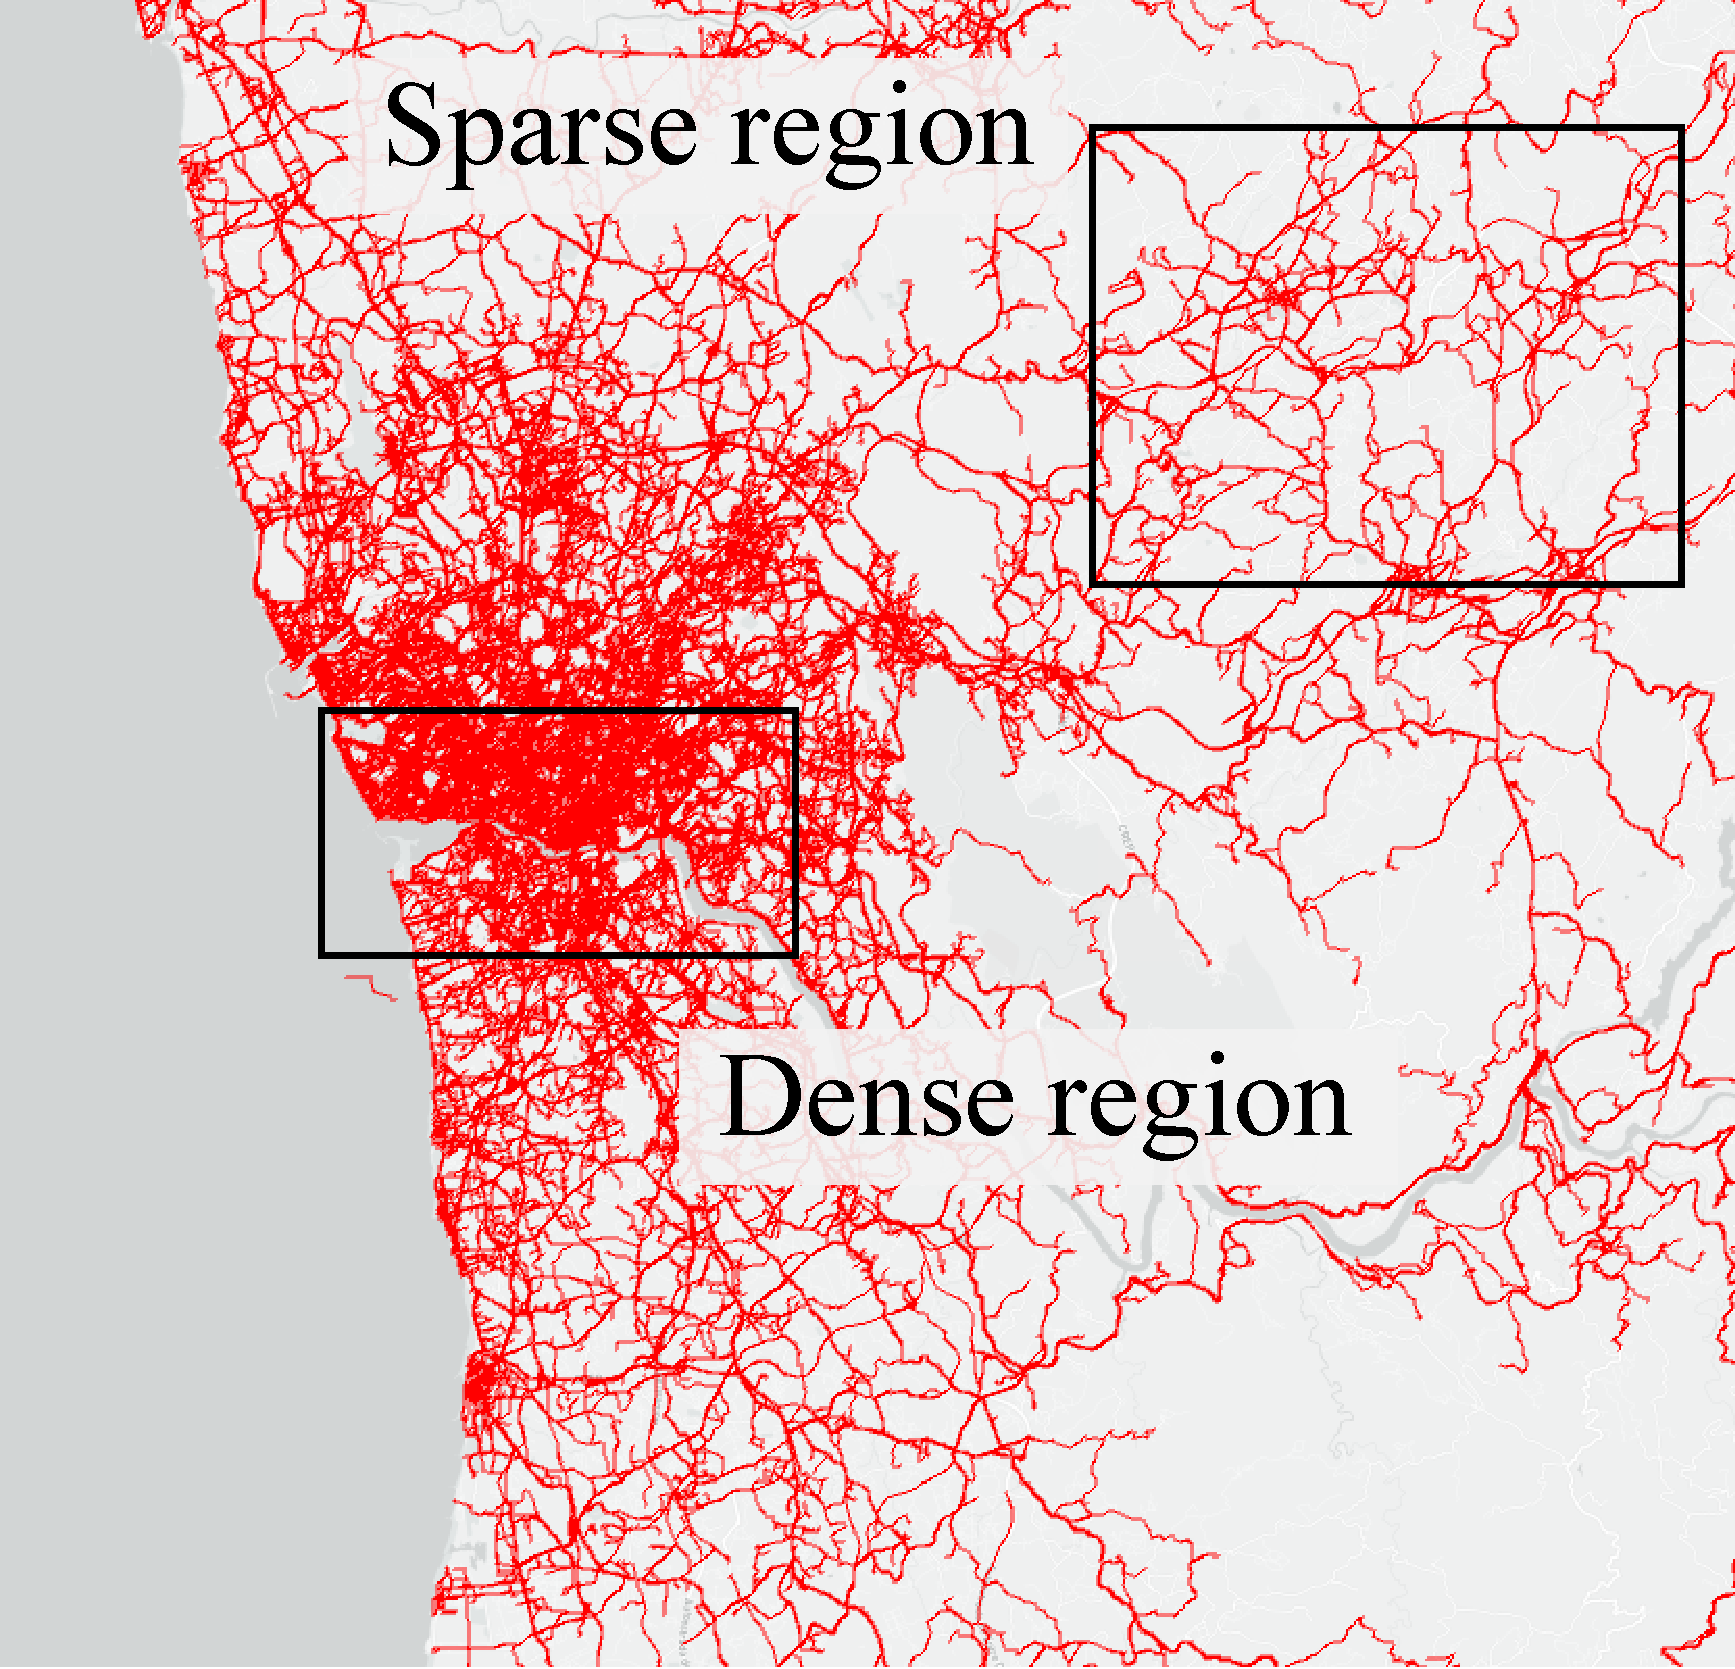
\includegraphics[width=0.250\linewidth]{pictures/motivation_VQGS+d64}
     &
     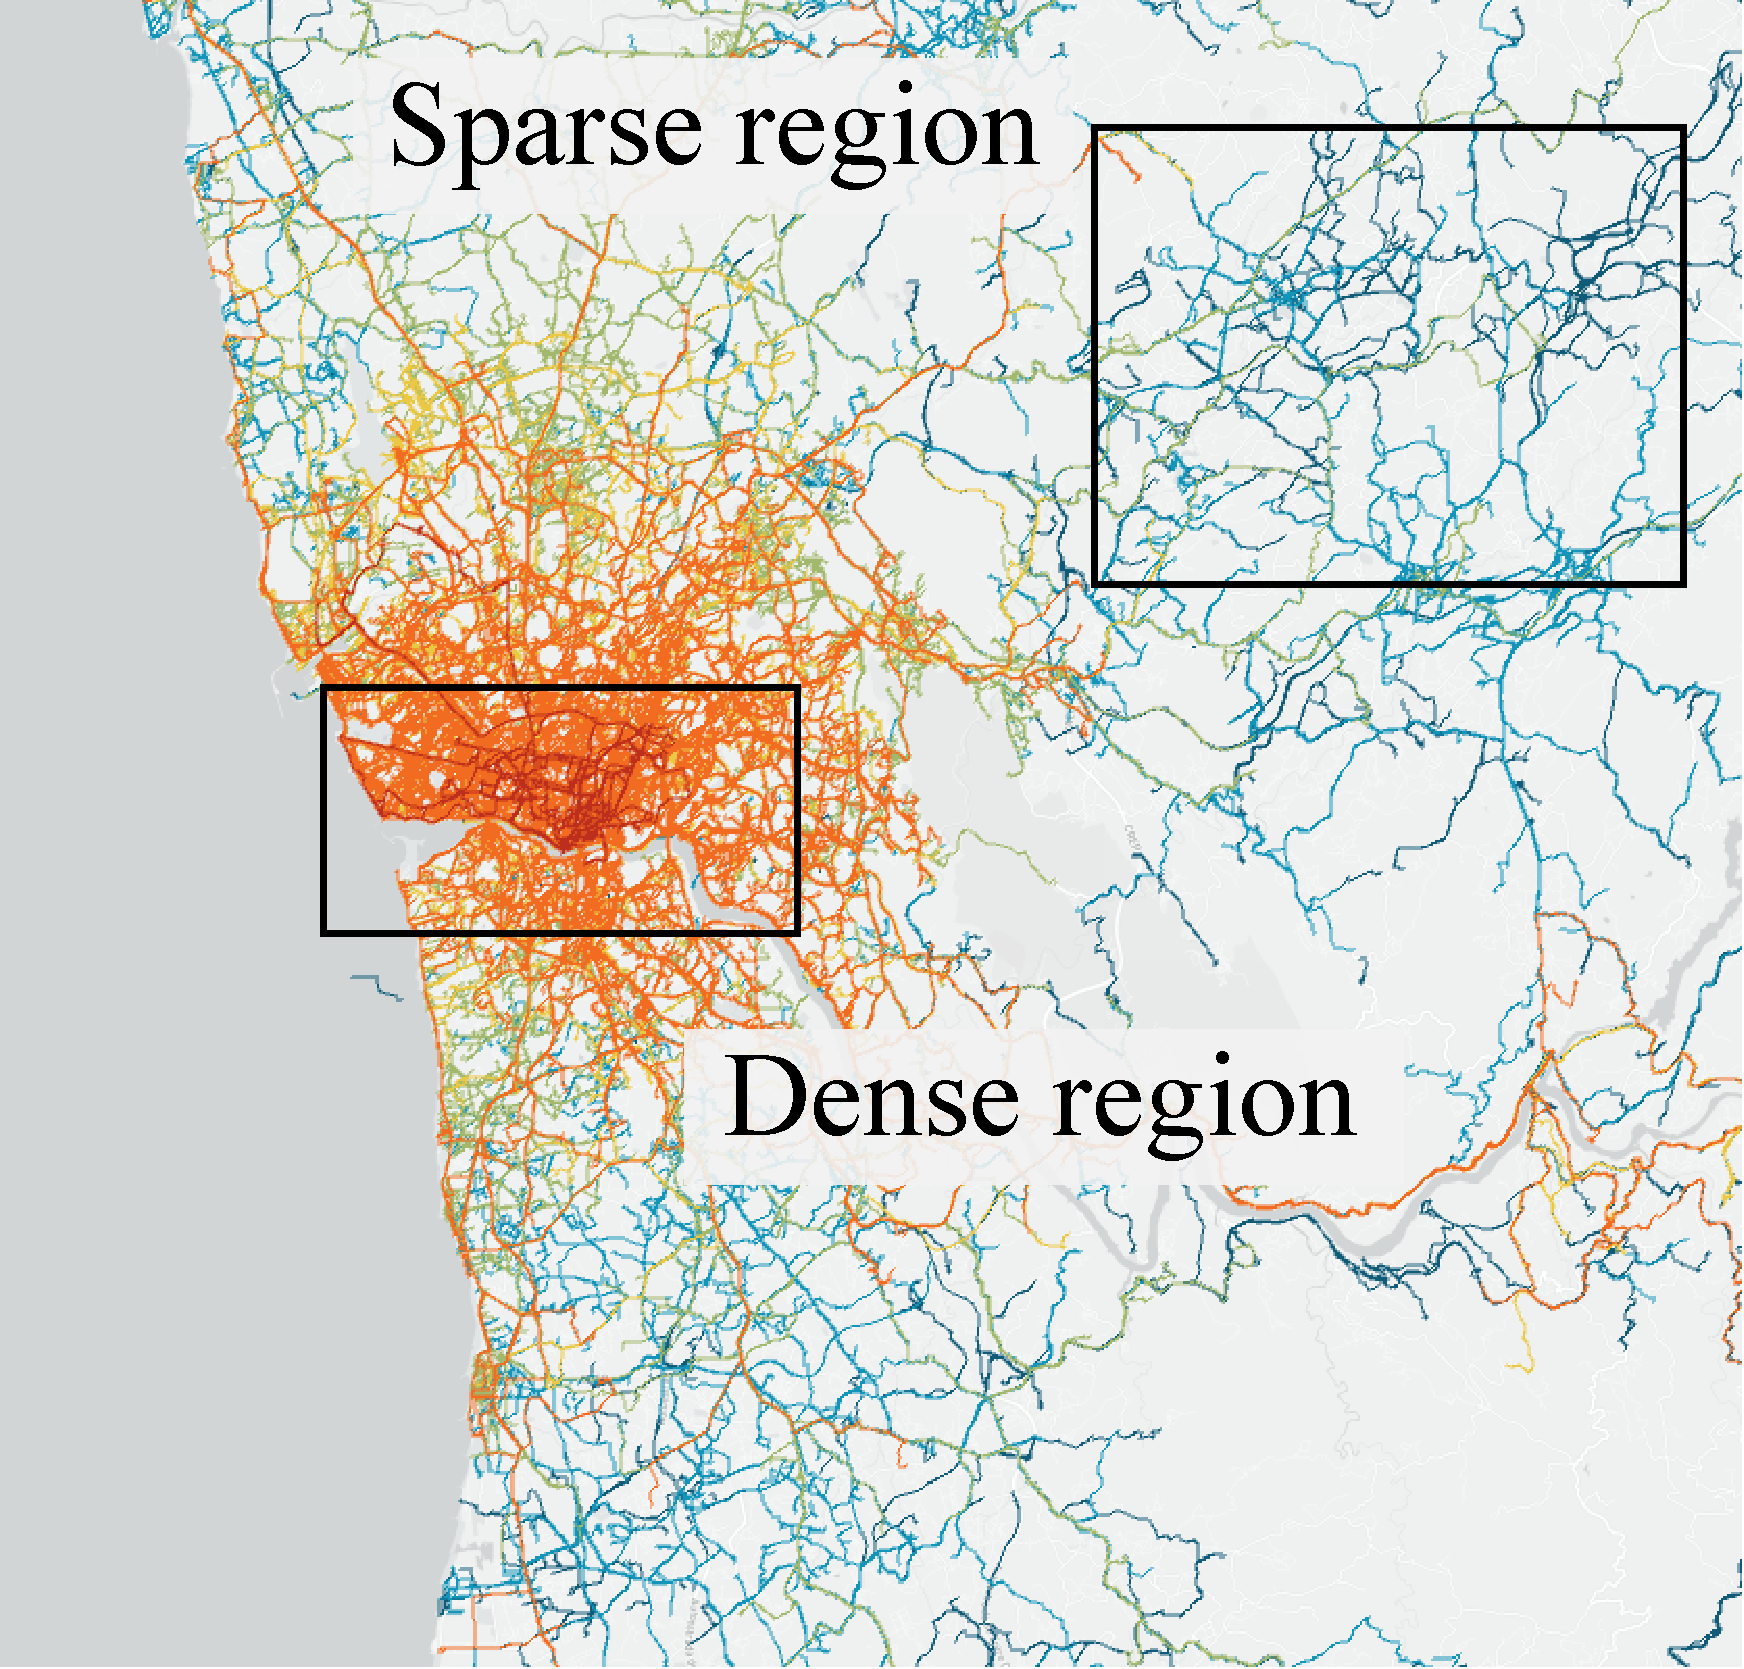
\includegraphics[width=0.250\linewidth]{pictures/motivation_VQGS+d64CE}
     \\
     (A) $\vats$
     &
     (B) $\vatss$
     &
     (C) $\vatssce$
     \end{tabular}
     \trim
     \caption{\prob{} solution $\vatss$ on \pt{} ($\alpha = 0.5\%, \delta = 64$)}\label{fig:delta}
   \end{minipage}\hfill
   \begin{minipage}{0.3\textwidth}
     \centering
     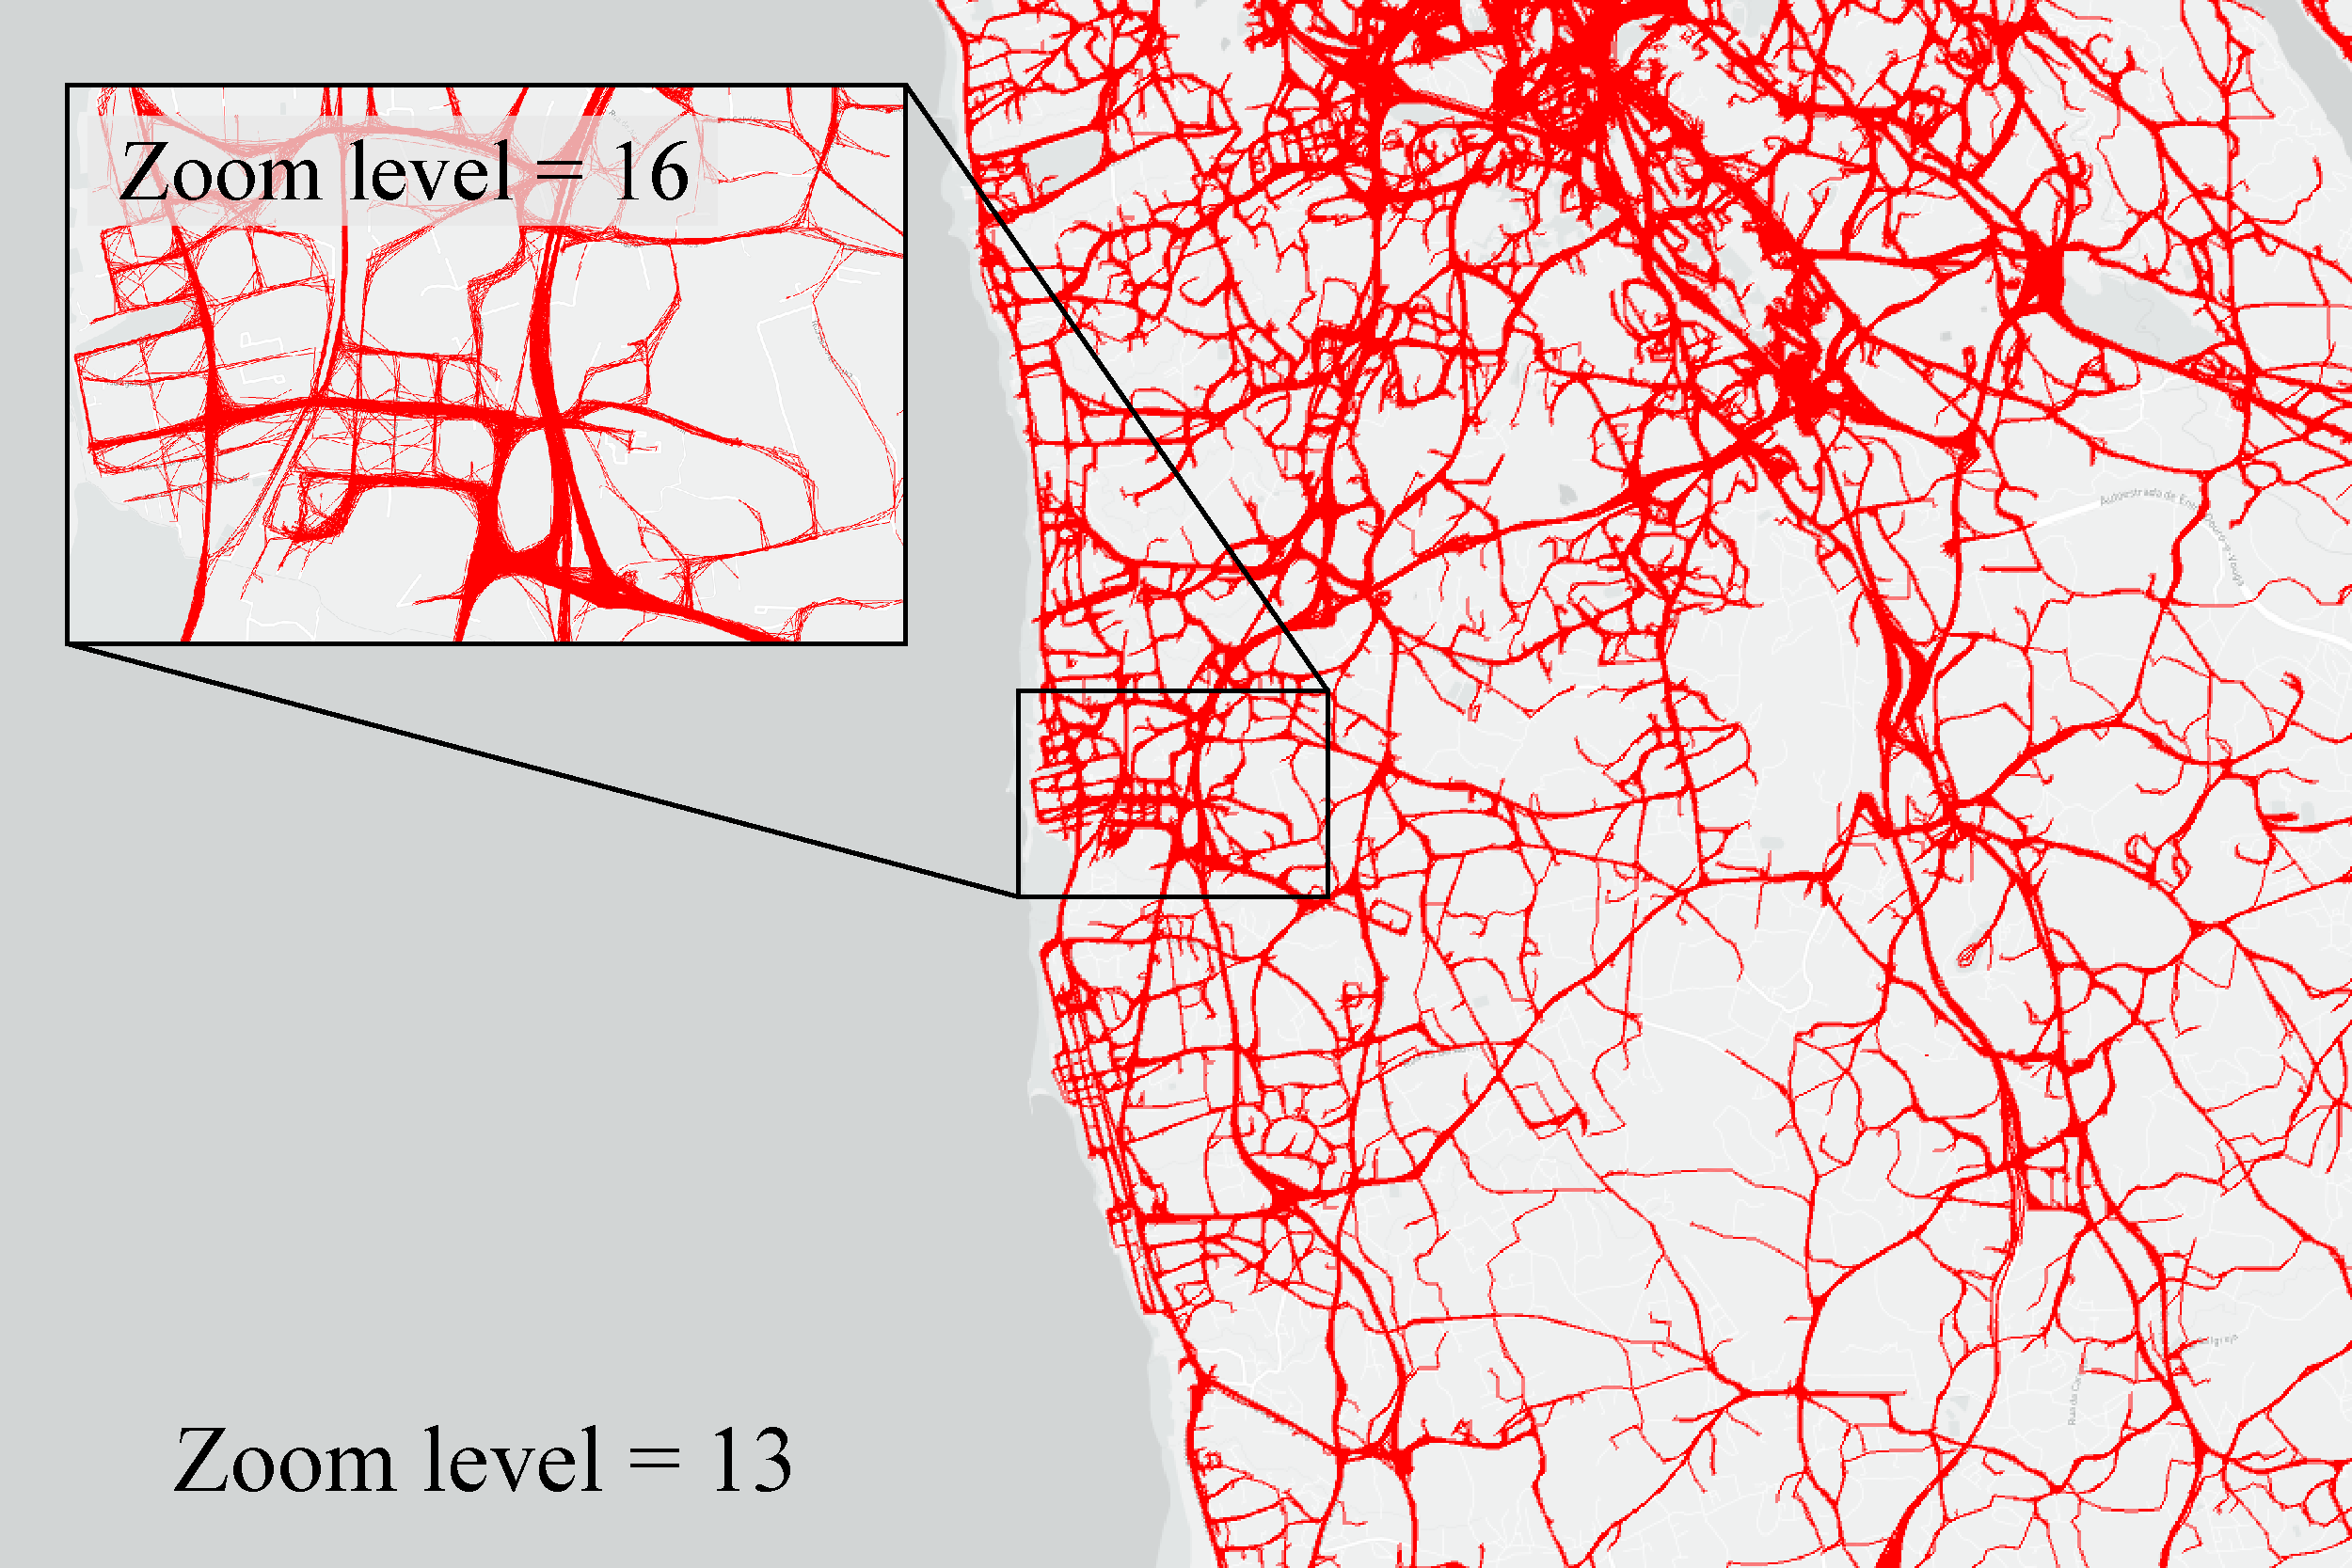
\includegraphics[width=0.85\linewidth]{pictures/zoomlevel.pdf}
     \label{Fig:zoom}
     \trim
     \caption{An illustration of different zoom level.}
   \end{minipage}
   \trim
\end{figure*}


%In the previous section, we presented the $\vats$ algorithm, which produces quality-guaranteed samples and runs efficiently. In this section, we focus on the third technical challenge: \emph{how to tackle the visual clutter problem in large trajectory visualization}?

In this part, we improve $\vats$ by considering (i) trajectory data distribution, and (ii) human perception capability. We elaborate (i) and (ii) by the examples in Figure~\ref{fig:delta}.


\stitle{Trajectory data distribution} Considering the \pt{} trajectory dataset, Figure~\ref{fig:delta}(A) is the visualization result of $\vats$ with sampling rate $0.5\%$.
It is obvious that the trajectories follow a non-uniform distribution, and there are some dense regions and sparse regions as illustrated by the two rectangles in Figure~\ref{fig:delta}(A).
There are many points in the dense region, which creates visual clutter and makes it difficult to identify the main roads.


%Obviously, the real-world trajectory dataset is non-uniform distributed.
%For example, the trajectories in dense region are much more than those in the sparse region, as illustrated by the rectangles in Figure~\ref{fig:delta}(A).

\stitle{Human perception capability} Comparing Figures~\ref{fig:delta}(A) and (B), it is easier to tell their differences in the sparse regions than in the dense regions.
This is because human perception has limited capability, and hence two visualizations look indistinguishable if both of them contain a large number of points in the same area.
The two dense regions look similar although Figure~\ref{fig:delta}(B) contain fewer points in this region than Figure~\ref{fig:delta}(A).
However, for the sparse region, $\vats$ loses some trajectories and it is easy to tell the differences between Figures~\ref{fig:delta}(A) and~\ref{fig:delta}(B).

%\begin{figure*}%[t]
%    \centering
%	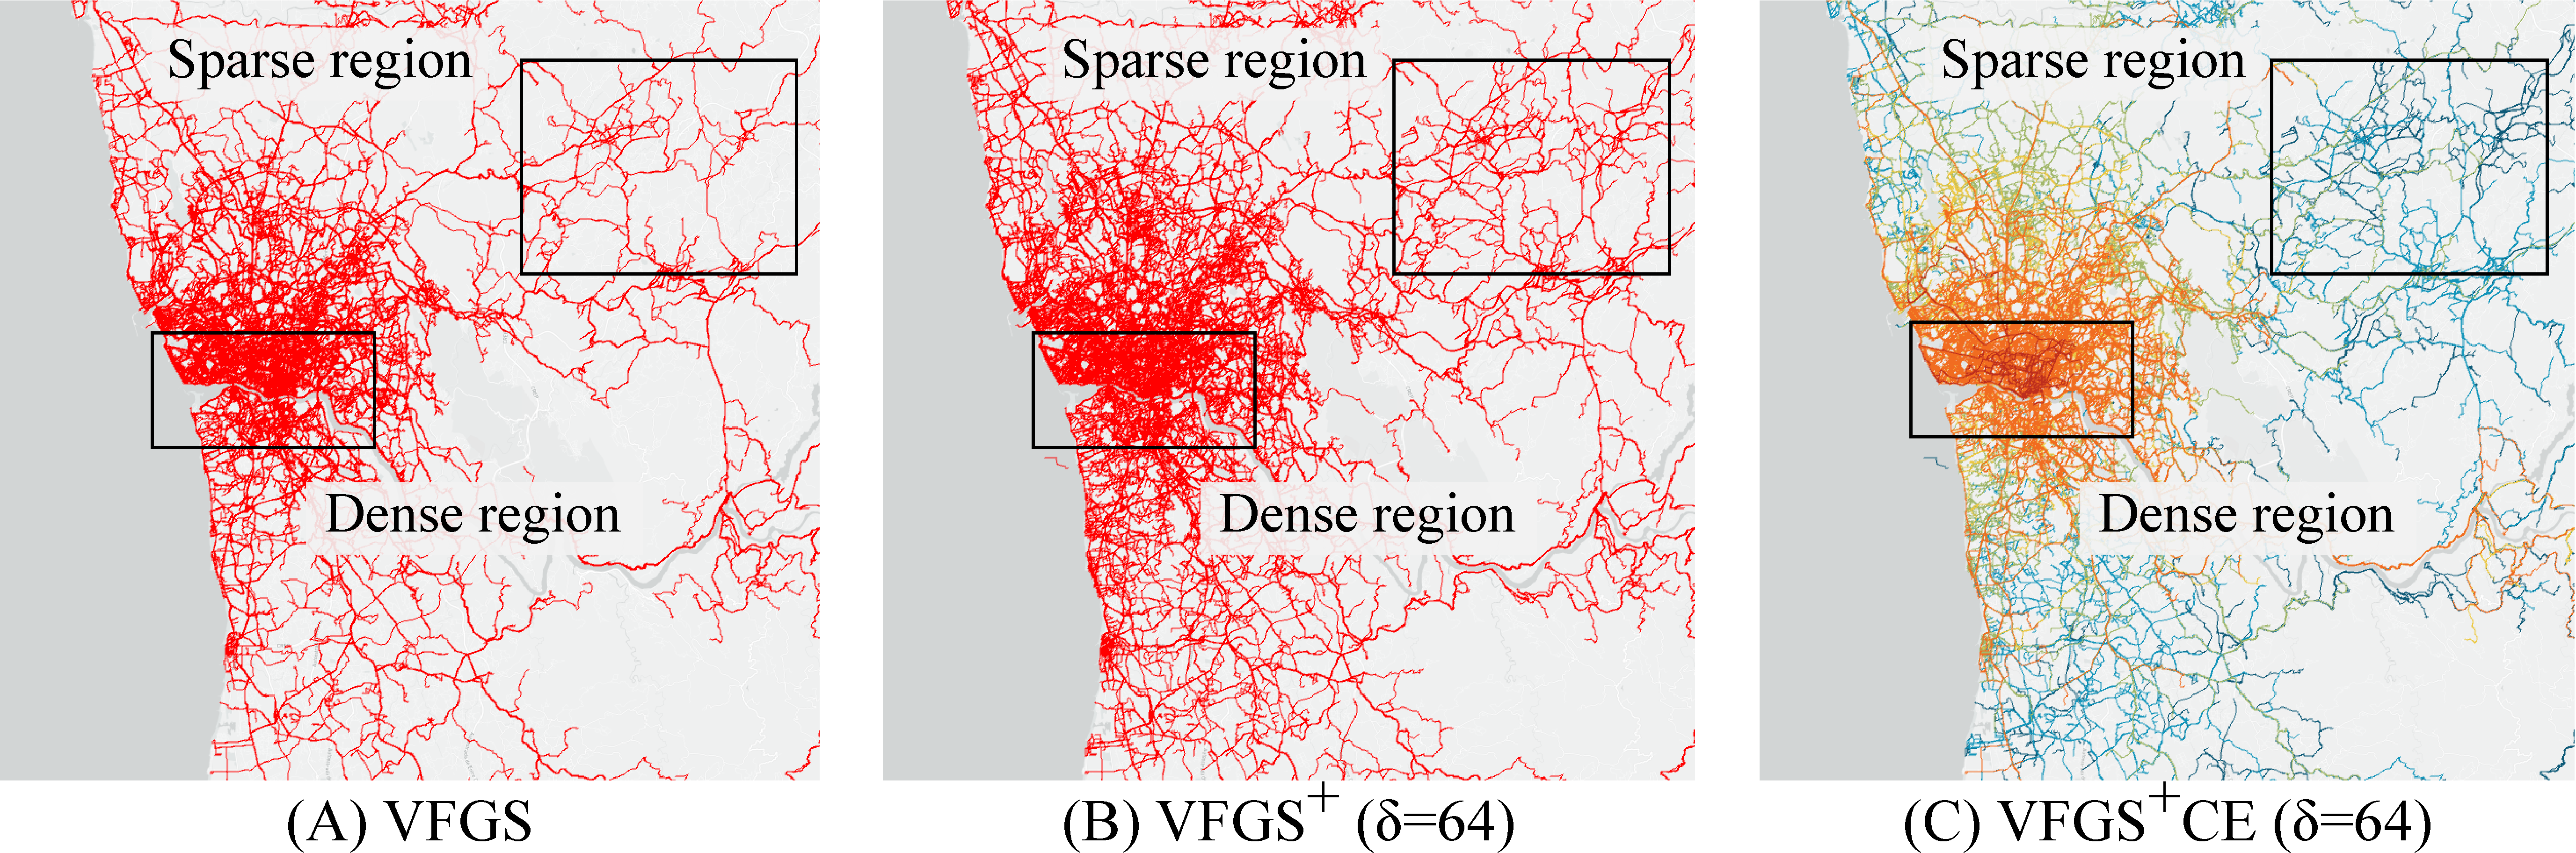
\includegraphics[width=0.7\textwidth]{pictures/problemsolveing/delta_motivation.pdf}
%	\caption{The advanced approach $\vatss$ on \pt{} ($\alpha = 0.5\%$).\Bo{edit figure captions}}\label{fig:delta}
%\end{figure*}


%\begin{table}
%  \begin{tabular}{cc}
%        \begin{figure}%[t]
%	       \centering
%	       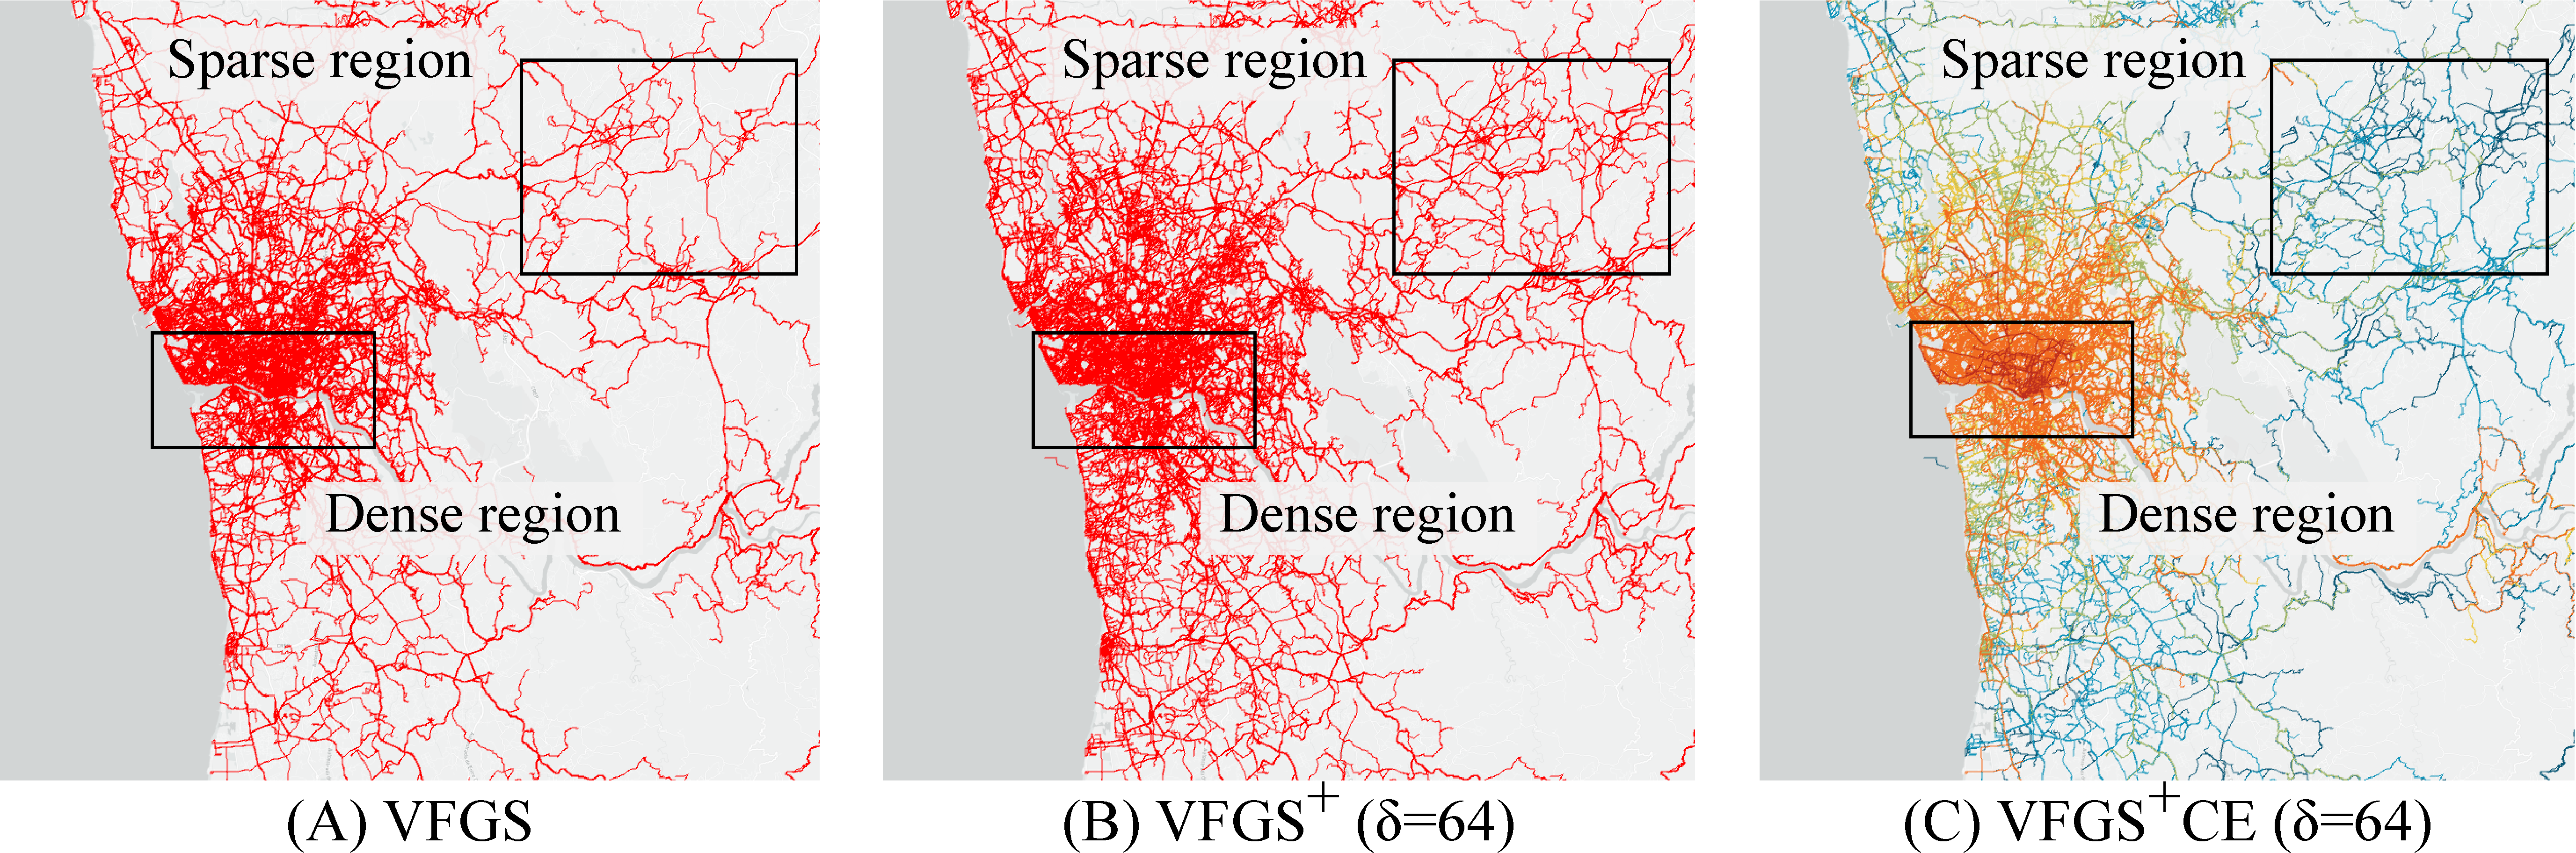
\includegraphics[width=0.7\textwidth]{pictures/problemsolveing/delta_motivation.pdf}
%	       \caption{The advanced approach $\vatss$ on \pt{} ($\alpha = 0.5\%$).\Bo{edit figure captions}}\label{fig:delta}
%        \end{figure}
%      &
%        \begin{figure}[t]
%        	\centering
%        	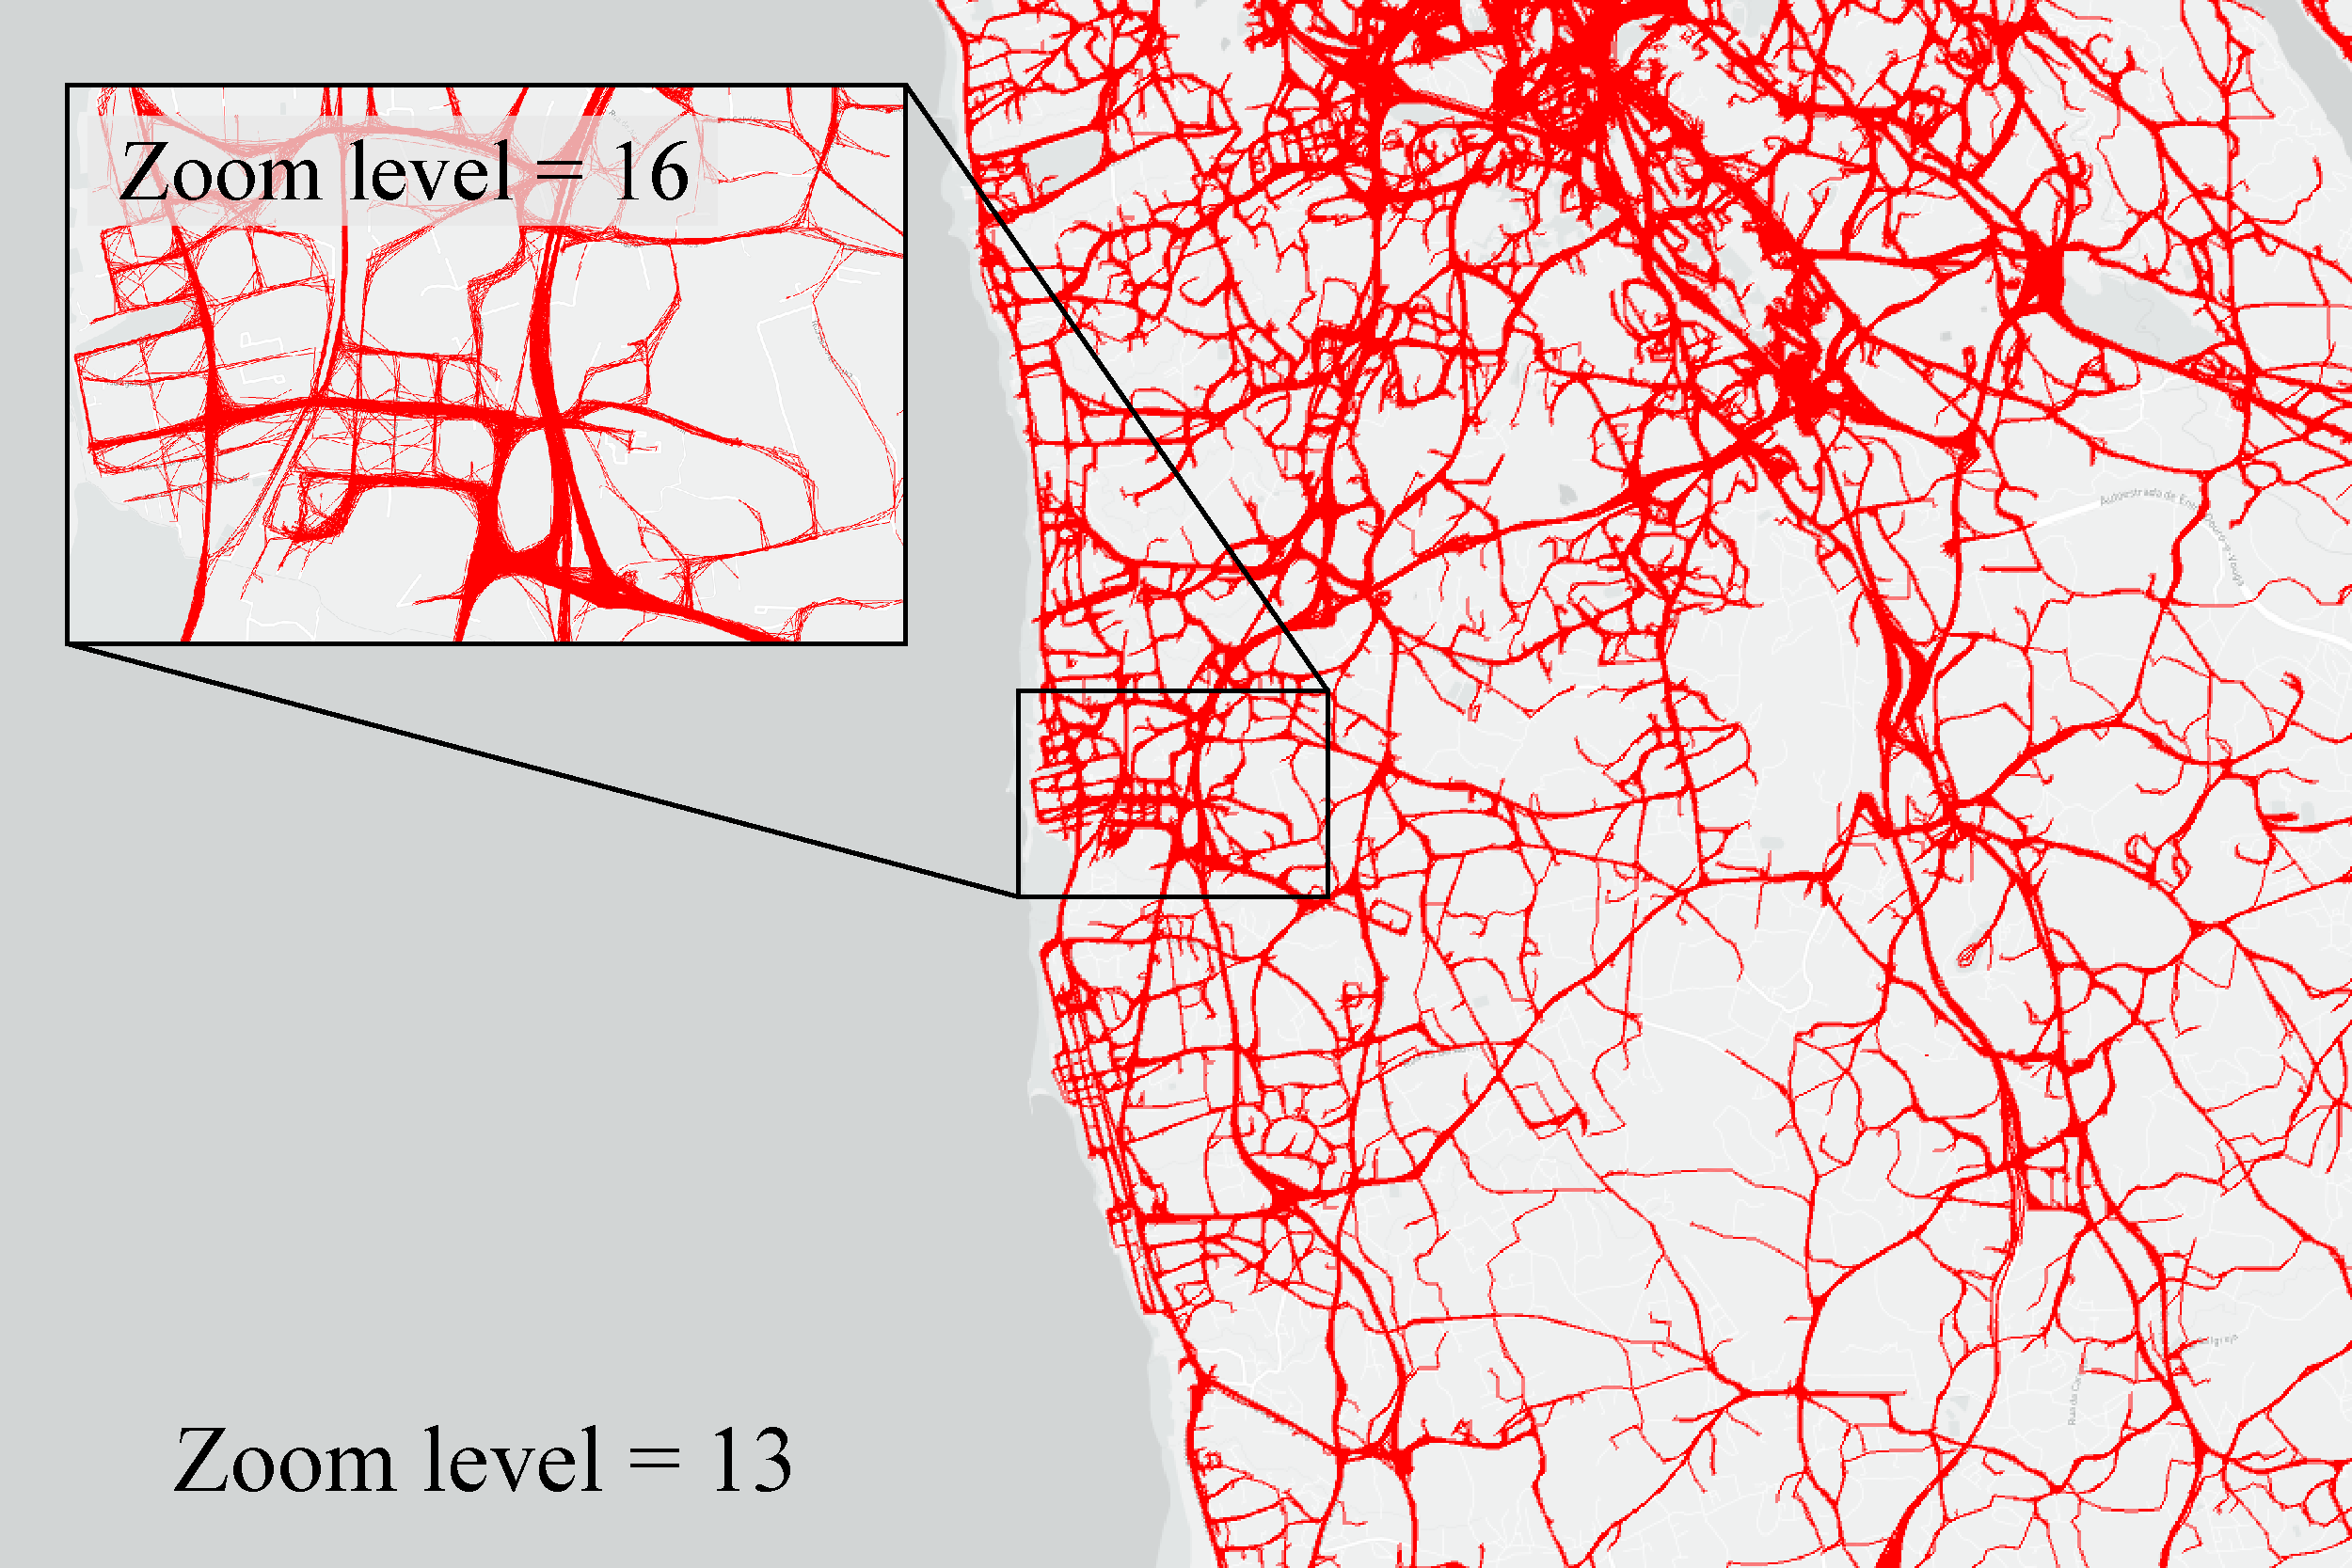
\includegraphics[width=0.3\textwidth]{pictures/zoomlevel.pdf}
%        	\caption{An illustration of different zoom level.}	\label{fig:zoom}
%        \end{figure}
%  \end{tabular}
%\end{table}



%(see Algorithm~\ref{alg:plus})

Based on the two observations above, we can improve  $\vats$ by delivering richer information in the sparse regions and reducing visual clutter in the dense regions.
$\vatss$ in Algorithm~\ref{alg:plus} achieves both objectives using a perception tolerance parameter $\delta$, which models the perception capability of humans.
Specifically, if pixel $(x,y)$ in the canvas is marked by the result set $\oR$,
the pixels around $(x,y)$, i.e., from $(x-\delta, y-\delta)$ to $(x+\delta, y+\delta)$, do not need to be marked as they are close to the pixels in $\oR$ and human perception cannot tell nearby pixels apart. We can easily modify $\vats$ in Algorithm~\ref{alg:greedy} to incorporate the perception tolerance parameter $\delta$ as shown in Algorithm~\ref{alg:plus}.
$\vatss$ measures the contribution of each trajectory $t_i$ w.r.t the augmented visualized point set $\VV(\oR)^{+}$ in Line~\ref{line:deltamax},
where $\VV(\oR)^{+}$ includes both pixels on the selected trajectories and their tolerance pixels (in Line~\ref{line:delta}).
We also use the heap-based lazy computation to speedup $\vatss$.


%Taking the above two observations into consideration, we can further improve the returning result of visual quality-guaranteed sampling approach $\vats$ by
%delivering rich information at sparse regions and reducing visual clutter in dense regions.
%In this section, we devise the advanced approach $\avats$ (see Algorithm~\ref{alg:plus}) to achieve the above two objectives.
%In specific, we introduce perception tolerance parameter $\delta$ in $\avats$, which models the perception capability of humans at the highest level of details.
%In other words, suppose the pixel $(x,y)$ in canvas is covered by the result set $\oR$ at the highest level,
%the pixels around $(x,y)$, i.e., from $(x-\delta, y-\delta)$ to $(x+\delta, y+\delta)$, are not necessary to cover because they are in the perception tolerance of human beings.


%It measures the contribution of each trajectory $t_i$ w.r.t the selected trajectory set $\oR$'s augmented set $\oR^{+}$, i.e., the selected trajectories and their tolerance pixels.
%.
%The augmented set $\oR^{+}$ will be updated by the selected trajectory $tmp$ and its tolerance pixels set (in Line~\ref{line:delta}).

%
\begin{algorithm}
    \caption{$\vatss(\D,k=\lceil \alpha \mathcal{T} \rceil,\delta)$} \label{alg:plus}
    \begin{algorithmic}[1]
    \State Initialize result set $\oR \leftarrow \emptyset$
    \State Initialize augmented result set $\oR^{+} \leftarrow \emptyset$
    \While{$|\oR| < k$}
        \State $\mathsf{tmp} \leftarrow \arg\max_{t_i \in \D} | t_i  \cup \VV(\oR)^{+} |$ \label{line:deltamax}
        \State $\oR \leftarrow \oR \cup \{ \mathsf{tmp} \}$
        \State $\VV(\oR)^{+} \leftarrow \VV(\oR)^{+} \cup \mathsf{augment}(\mathsf{tmp}, \delta)$\label{line:delta}
    \EndWhile
    \For{each $t$ in $\D$} \Comment{Representative encoding} \label{line:s}
        \State $tr \leftarrow \arg\min_{t_i \in \oR}{|t-\mathsf{augment}(t_i, \delta)|}$
        \State $tr.\mathsf{cnt}++$ \label{line:e}
    \EndFor
    \State Return $\oR$
    \end{algorithmic}
\end{algorithm}


%Interestingly, the visual clutter large trajectory visualization problem can be further reduced
%by encoding representative trajectories in $\oR$ (the returning result of $\avats$) with colors.
%In particular, $\avats$ selects the trajectory with the largest uncovered pixels by taking the perception tolerance capability of humans into account at each iteration,
%instead of only choosing the trajectory with the largest uncovered pixels in $\vats$ (Algorithm~\ref{alg:greedy}).


$\vatss$ in Algorithm~\ref{alg:plus} selects trajectories with good representativeness and some trajectories will not be included into the result set $\oR$ even though they have more uncovered pixels w.r.t. $\oR$.
The reason is that their uncovered pixels are too close to the pixels in the selected trajectories (i.e., within the tolerance area of selected pixels).
Compared with $\vats$, $\vatss$ is more likely to sample trajectories in the sparse regions as their pixels are less likely to be covered by other trajectories as shown in Figures~\ref{fig:delta}.
Moreover, reducing the number of trajectories sampled from the dense regions helps to reduce visual clutter.


%Take Figure~\ref{fig:zoom}(A) for example, suppose $\delta=1$ and trajectory $a$ was selected at the first iteration, the trajectory to select in the second iteration is $c$ instead of $b$ because almost all pixels in $b$ is in the tolerance area of $a$'s.

%\begin{figure}[t]
%	\centering
%	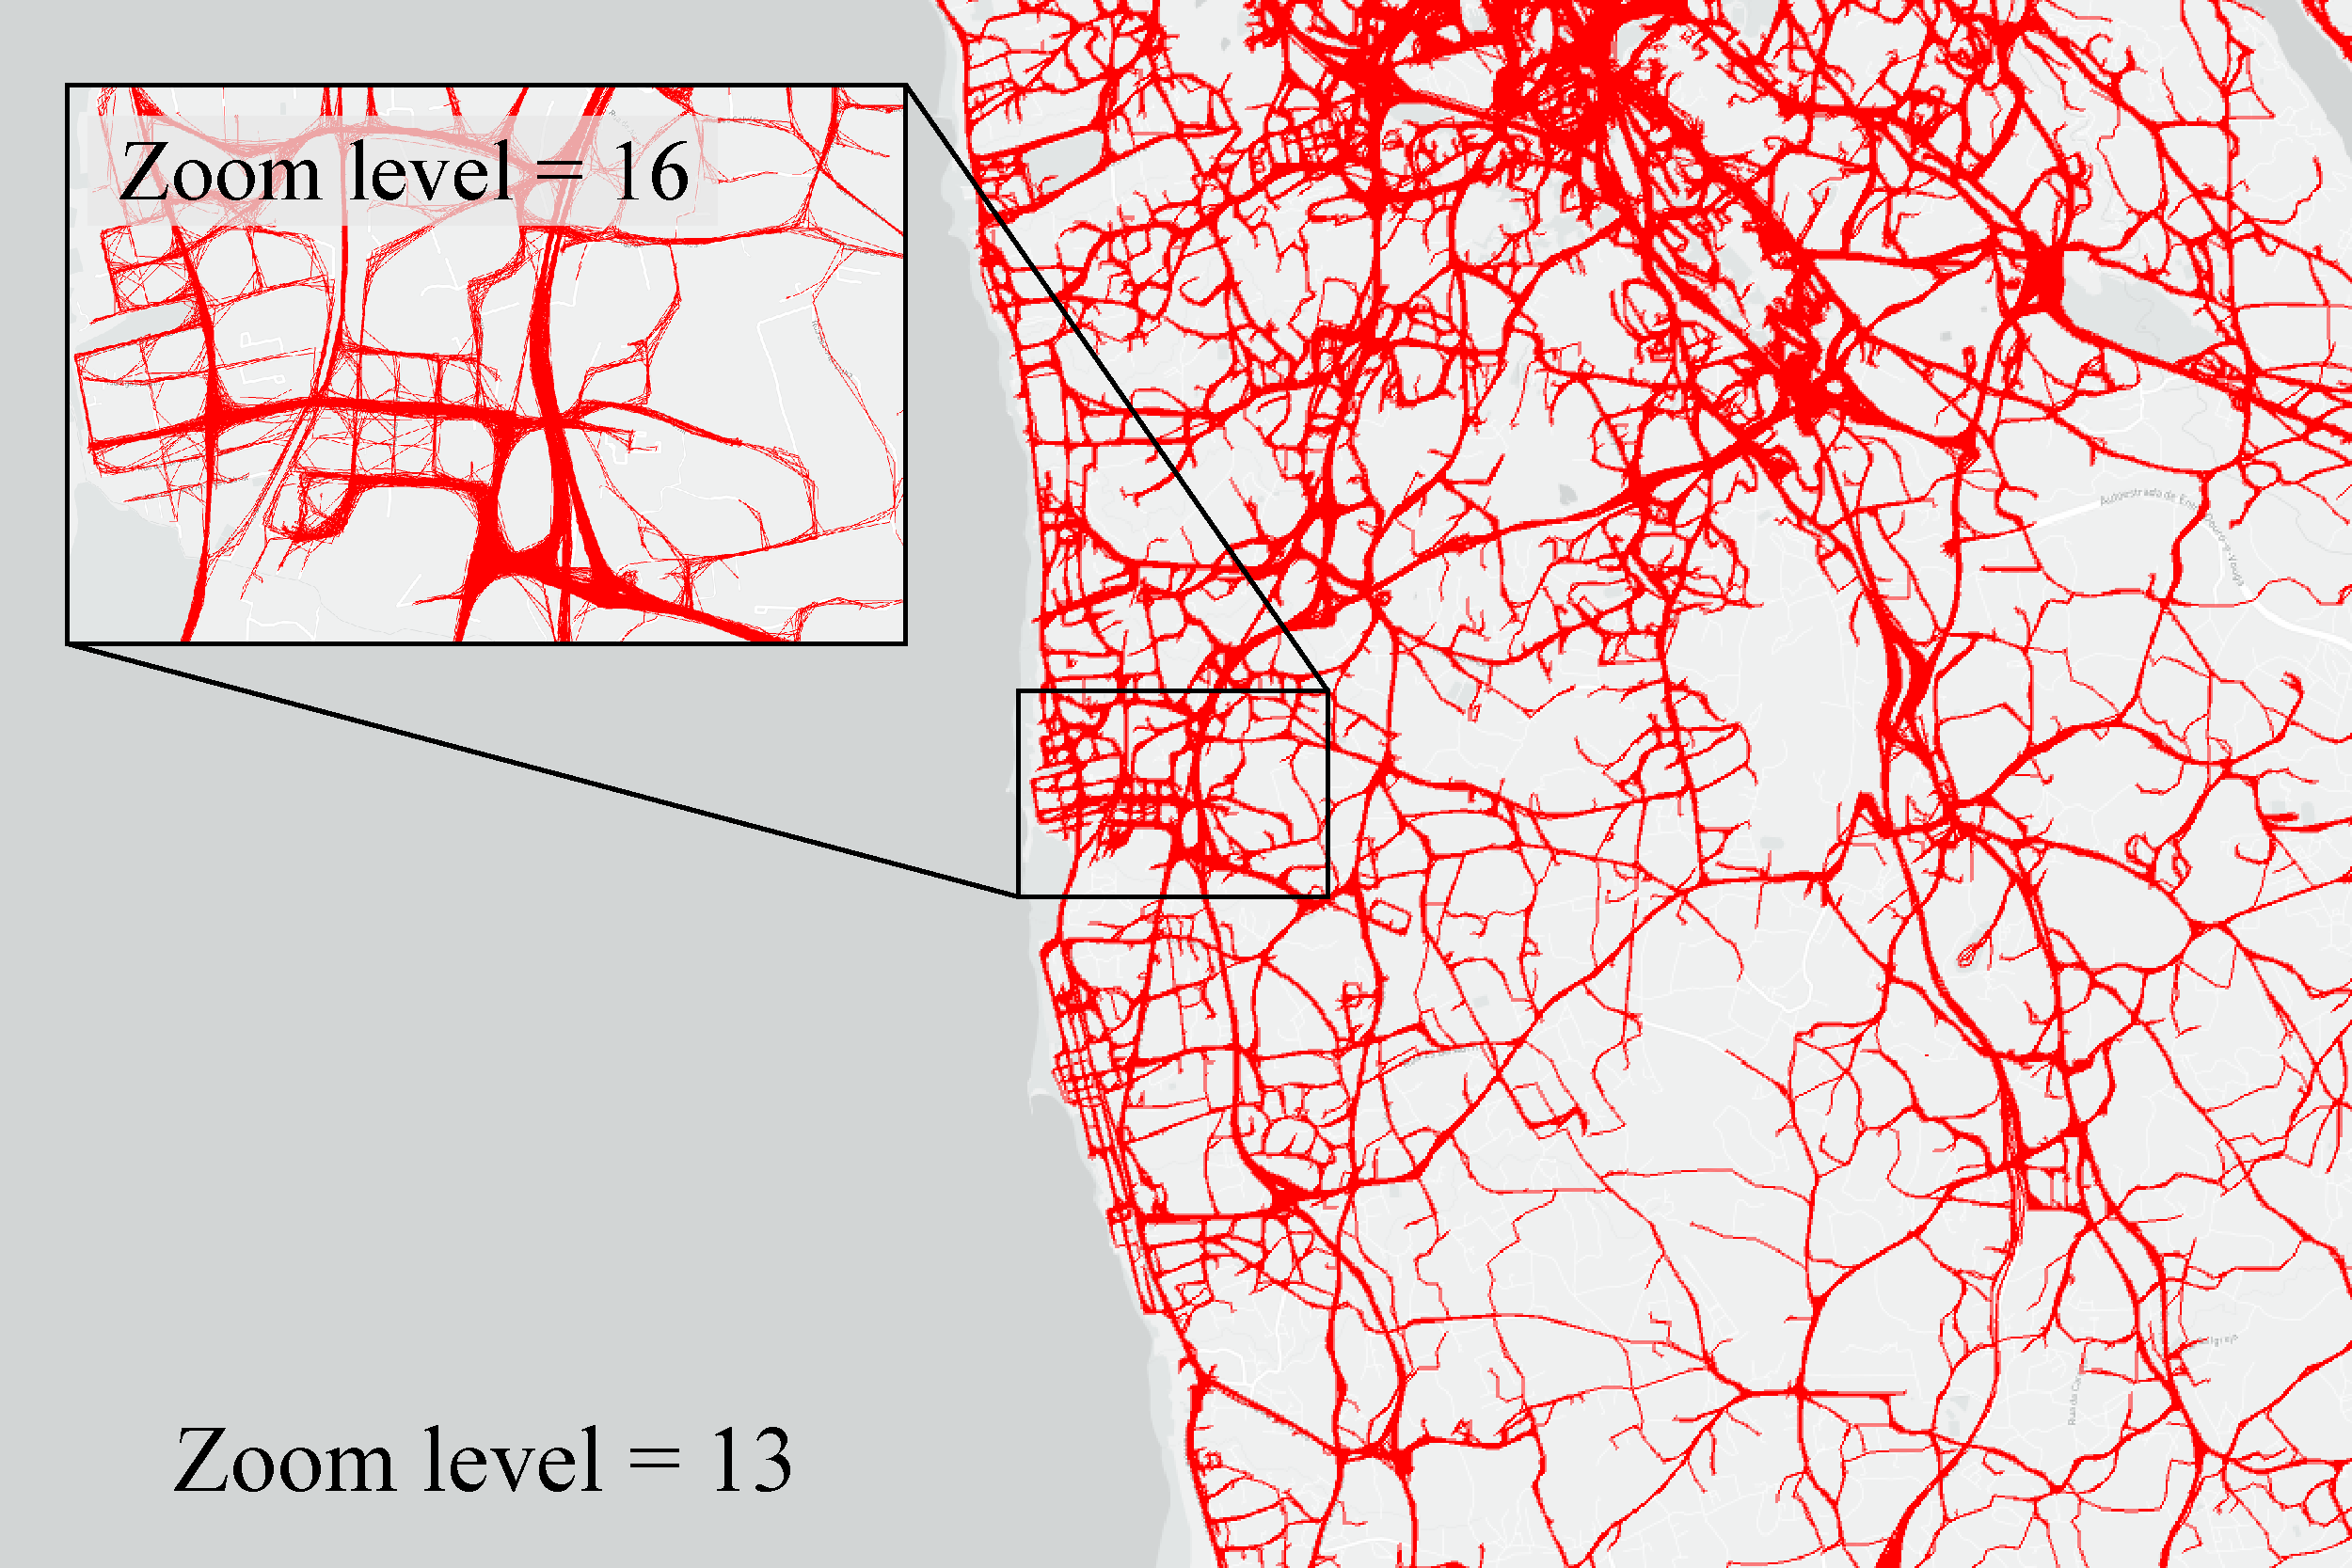
\includegraphics[width=0.3\textwidth]{pictures/zoomlevel.pdf}
%	\caption{An illustration of different zoom level.}	\label{fig:zoom}
%\end{figure}


One subtlety is that different $\delta$ needs to used for different \emph{zoom levels} (or regions with different sizes).
For example, Google map~\cite{googlemap} provides zoom levels from 0 to 20, with level 0 providing the largest visualization range (i.e., the whole world) but the lowest resolution, and level 20 providing the smallest visualization range (e.g., individual building, if available) but the highest resolution.
We provided an illustration of zoom level in Figure 6 and users may select different zoom levels for visualization according their needs.
Note that we define $\delta$ on the highest zoom level (i.e., using the raw distance of the locations) to account for different resolutions.
If the zoom level is small (i.e., the visualization region is large), we can apply a large $\delta$ because locations with a large raw distance look close to each other in the visualization and we can afford to lose more details.
If the zoom level is large (i.e., the visualization region is small), we need to use a small $\delta$ as users typically want to investigate some fine-grained details in this case and using a large $\delta$ will lose these details.

%We will elaborate this point shortly in experimental section.

%Therefore, we use different $\delta$ for different zoom levels accordion to Table~\ref{tab:delta}, which was obtained empirically from a user evaluation of the visualization results.
%\begin{table}
%	\centering
%	\small
%	\caption{Values of $\delta$ for different zoom levels}
%	\begin{tabular}{|c|c|c|c|c|} \hline
%		\textbf{Zoom Level} &  &  &  & \\
%		\hline
%		$\delta$ &  &  & &  \\ \hline
%	\end{tabular}	\label{tab:delta}
%\end{table}

%Ideally, we want a sample to be \textit{zoom-level-independent}, providing a consistent quality guarantee at different zoom levels. This turns out to be straightforward as trajectory visualization merges several pixels in a high-level result (by pixel-wise $OR$) to obtain a pixel in a lower-level visualization result. The following theorem shows that it suffices to satisfy the quality guarantee at the highest zoom level.

%$\delta$ for different zoom levels, user study smaller delta for higher zoom levels


%$\vatss$ also provides excellent visual quality at arbitrary zooming resolutions. This is because it considers the perception tolerance parameter $\delta$  at the highest zoom level. For example, the zoom level in Figure~\ref{fig:zoom}(A) is higher than that in Figure~\ref{fig:zoom}(B). According to our elaboration, $\vatss$ selects trajectory $a$ and $c$ for Figure~\ref{fig:zoom}(A). When the area is zoomed out, as shown in Figure~\ref{fig:zoom}(B), trajectory $a$ and $c$ still captures the main sketch of the underlying dataset (as gray cells shown).





\stitle{Color encoding scheme}
The visual clutter problem for large-scale trajectory visualization can be further alleviated by encoding the representativeness of the trajectories in $\oR$ with colors.
We define the representativeness of a trajectory $t_i$ in $\oR$ as the size of its \emph{reverse nearest neighbor set}, which contains the trajectories in $\D$ that has $t_i$ as its nearest neighbor in $\oR$.
The distance between trajectory $t$ and $t_i$ is defined as the number of pixels in $t$ that can not be covered by the augmented pixels of $t_i$.
We compute the representativeness of each trajectory in $\oR$ in Lines~\ref{line:s}-\ref{line:e} in Algorithm~\ref{alg:plus}.
Figure~\ref{fig:delta}(C) shows the visualization result by encoding trajectories with larger representativeness with warmer colors. Compared with Figure~\ref{fig:delta}(B), the main roads in the dense region is clearer in Figure~\ref{fig:delta}(C) with very warm colors.

%There are more details in the sparse regions compared with the $\vats$ result in Figure~\ref{fig:delta}(A), and we can identify the main roads in the dense region with very warm colors.

%Thus, the selected trajectories in the dense region are more representative than those in sparse region.



%		&
%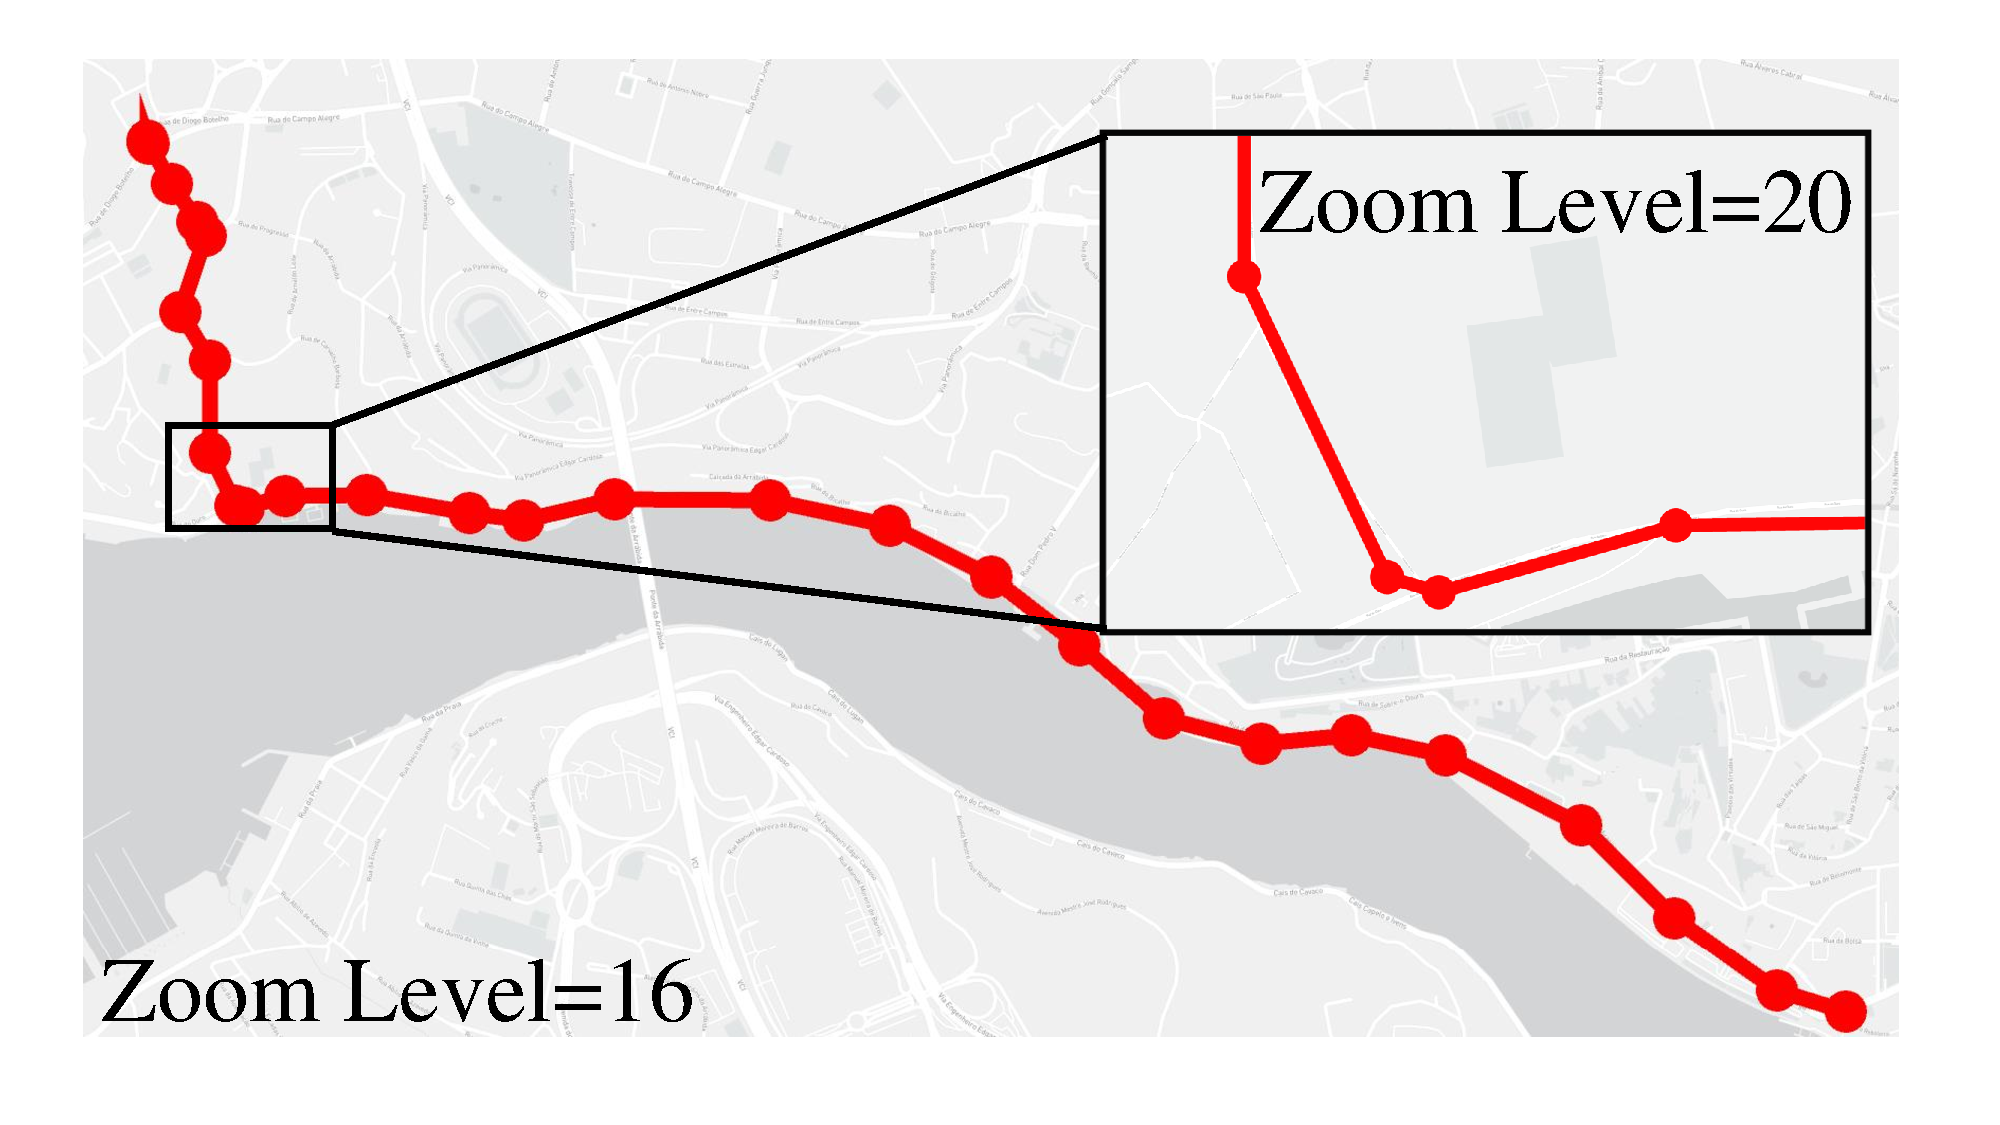
\includegraphics[width=0.48\columnwidth]{pictures/problemsolveing/TrajZoomIn}		
%\\
%(A) Line-based visualization
%&
%(B) Zoom levels


%(1) Richer Information Delivering: details aware; so Arbitrary zooming resolutions
%(2) Popularity Embedding: visual clutter



%\subsection{One-to-many strategy}~\label{sec:one_to_many}
%Since we detect the covered pixels in the highest level, two trajectories may be very close to each other but share very few pixels, which will lead to more information loss in the low zoom view as figure~\ref{fig:one_to_many}.
%We next elaborate a ``one-to-many'' strategy to further optimize the visual quality of our proposed technique.
%Recalling we use the highest zoom level to define the pixel size in the canvas.
%Thus, our visual quality guaranteed sampling algorithm is zoom-level oblivious, e.g., it guarantees the visual quality of result set $\oR$ at every zoom level.
%However, users always do not use/need the highest zoom level in visualization applications.
%For example, Google map shows city and streets at zoom level 1 and 15, respectively~\footnote{\url{https://developers.google.com/maps/documentation/}}.
%Motivated by the above observation, we devise ``one-to-many'' strategy by introducing a visual tolerance parameter $\delta$ to optimize the visual quality for users.
%Specifically, ,
%the ``one-to-many'' strategy will ignore all the pixels around $(x,y)$ within $\delta$ offset distance, i.e., all pixels from $(x-\delta, y-\delta)$ to $(x+\delta, y+\delta)$ will be skipped.
%We will demonstrate the effectiveness of the visual tolerance $\delta$ in experimental evaluations.
%
%%https://developers.google.com/maps/documentation/maps-static/dev-guide#Zoomlevels
%\begin{figure}[t]
%	\centering
%	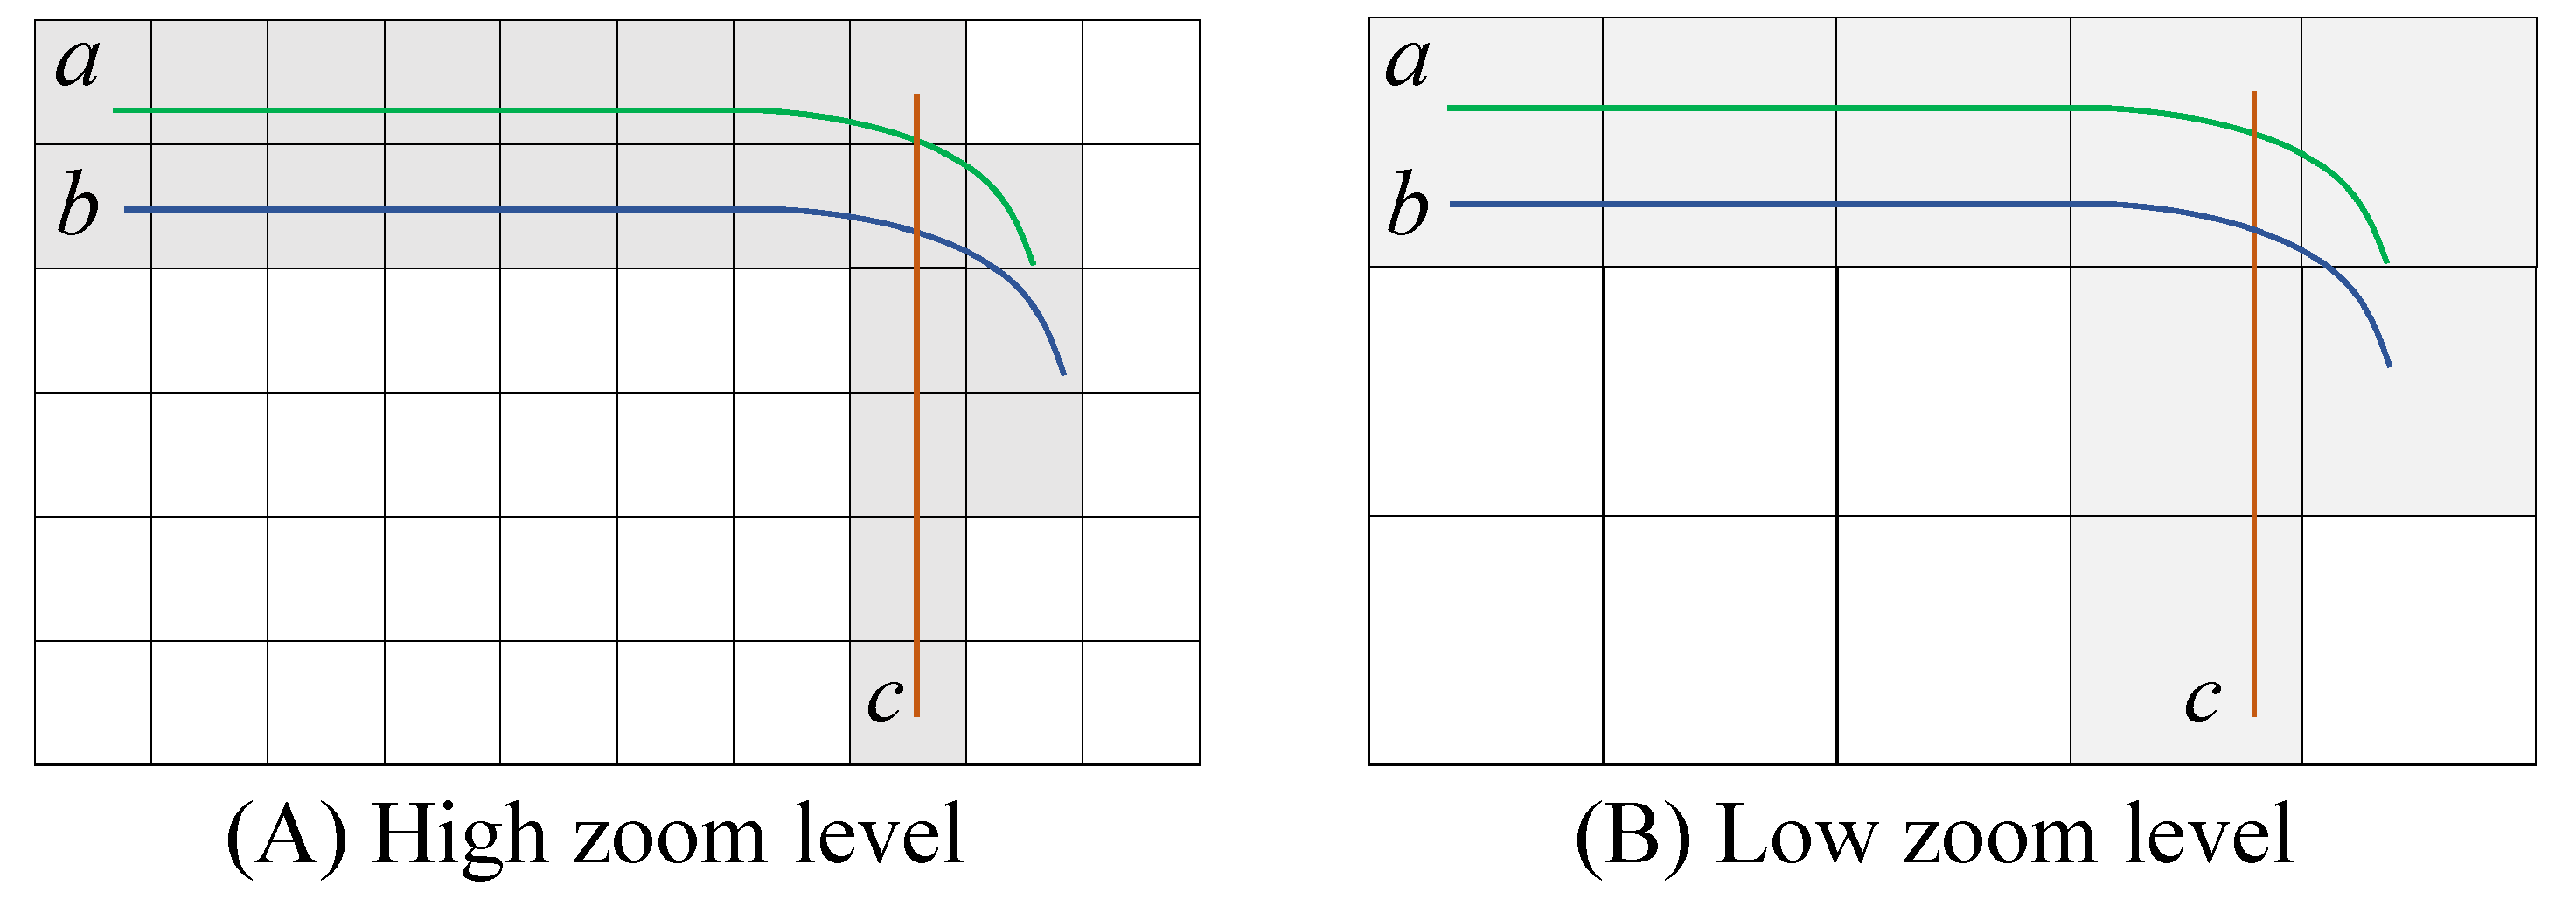
\includegraphics[width=0.4\textwidth]{pictures/problemsolveing/one_to_many.pdf}
%	\vspace{-5mm}
%	\caption{Resolution inconsistency}
%	\vspace{-5mm}
%	\label{fig:one_to_many}
%\end{figure}


%Specifically, $\avats$ incorporates a parameter $\delta$ during trajectory selection process in $\vats$ .
%In particular, we employ the parameter $\delta$ to model the end user's perception ability at the most high level of details.
%Surprisingly, our advance approach $\avats$ not only provides better visualization result when comparing with $\vats$ with the same sampling rate
%(e.g., Figure~\ref{fig:delta}(a) and (b) are the returning result of $\vats$ and $\avats$ respectively),
%but also embeds the popularity of selected trajectories by encoding the rest trajectories in the dataset in them,
%e.g., Figure~\ref{fig:delta}(c) is the visual result of $\avats$ with color encoded popularity.



